%\documentclass[10pt,a4paper]{scrartcl}
\documentclass[10pt,a4paper,cleardoubleempty]{scrbook}

%\documentclass[]{scrreprt} % classe report di KOMA-Script
%\documentclass[h. . .i]{scrbook} % classe book di KOMA-Script
\usepackage{}
\usepackage[]{classicthesis-ldpkg}
\usepackage[parts,linedheaders,pdfspacing]{classicthesis}
\usepackage[italian]{babel}
\usepackage[utf8]{inputenc}
\usepackage{graphicx}
\usepackage{indentfirst}

\hypersetup{pdfborder={0 0 0}}

\usepackage{allrunes}

\usepackage{color}
\definecolor{Brown}{cmyk}{0,0.81,1,0.60}
\definecolor{OliveGreen}{cmyk}{0.64,0,0.95,0.40}
\definecolor{CadetBlue}{cmyk}{0.70,0.57,0.23,0}

% includes official (and very dirty) stuff
%\usepackage{Official/uniudtesi}
\hypersetup{
    pdftitle={Sviluppo di Strumenti didattici per la programmazione Embedded},
    pdfauthor={Michele Bianchi},
    pdfsubject={Sviluppo blocchi per SciCos},
    pdfkeywords={NXT, nxtOSEK, SciCosLab}
}
\usepackage{makeidx}
\makeindex
%\usepackage{fancyhdr}
\fancyhf{}
\fancyhead[LE,RO]{\bfseries\thepage}
\fancyhead[LO]{\bfseries\rightmark}
\fancyhead[RE]{\bfseries\leftmark}
\renewcommand{\headrulewidth}{0.5pt}
\renewcommand{\footrulewidth}{0pt}



\usepackage[final]{pdfpages}


\usepackage{listings}
\lstset{language=[ansi]C,
        frame=tRBl, %
        frameround=ftff, %
        basicstyle=\footnotesize, %
        keywordstyle=\ttfamily\color{OliveGreen}, %
        identifierstyle=\ttfamily\color{CadetBlue}\bfseries, %
        commentstyle=\slshape\ttfamily\color{Brown}, %
        stringstyle=\ttfamily, %
        showstringspaces=true, %
        captionpos=b
}

\lstset{
    morekeywords={U8, S8, U16, S16, U32, S32, bool, size_t, uint8_t,
    uint16_t, uint32_t, int8_t, int16_t, nx_bmp_t, int32_t,
    nx_rs485_error_t, nx_rs485_baudrate_t, nx_aic_priority_t, action_t,
    nx_struct, nx_uint8_t, nxt_protocol_header_t, nx_union, nxle_int8_t,
    nxle_uint32_t, nxle_uint16_t, nxle_int16_t, nxt_protocol_t, action_t,
    atomic, norace, command, event, error_t, signal, call, task, post,
    configuration, implementation, components, as, module, interface,
    uses, provides, bro_bt_device_t, bdaddr_t, scicos_block}
}

\renewcommand*\lstlistingname{Listato}

\newenvironment{code}[2]{       %
    \lstset{caption=#1,label=#2}%
    \begin{lstlisting}}         %
    {\end{lstlisting}}

% args: image path
%       caption
%       width
%       label
\newcommand{\image}[4]{%
    \begin{figure}[hbt]%
    \centering%
    \includegraphics[width=#3\columnwidth]{#1}%
    \caption{\emph{#2}}%
    \label{#4}%
    \end{figure}%
}

% args: image path
%       caption
%       label
\newcommand{\imageFullWidth}[3]{\image{#1}{#2}{0.8}{#3}}

\newcommand{\picref}[1]{figura \ref{#1}}

\newcommand{\website}[2]{Sito web di \techname{#1}: \\ \url{#2}}
\newcommand{\paper}[3]{#1: \emph{#2} \\ \url{#3}}

\newcommand{\techname}[1]{{\sc #1}}

\newcommand{\nxt}{\emph{Lego MINDSTORMS NXT}}
\newcommand{\nxtOSEK}{\emph{nxtOSEK}}
\newcommand{\BROFist}{\emph{BROFist}}
\newcommand{\SPAM}{\emph{SPAM}}
\newcommand{\PID}{\emph{Digital PID Controller}}
\newcommand{\RIS}{\emph{Robotics Invention System}}

\usepackage{}
\author{Michele "Jazzinghen" Bianchi}
\title{Sviluppo di Strumenti didattici per la programmazione Embedded}
\begin{document}

    %\begin{titlepage}
\begin{center}
\LARGE{UNIVERSIT\`A DEGLI STUDI DI TRENTO\\}
\large{Facolt\`a di Scienze Matematiche, Fisiche e Naturali\\}
\begin{figure}[ht]
    \begin{center}
        
\includegraphics[scale=0.25]{official/logo}
    \end{center}
\end{figure}
Corso di Laurea triennale in Informatica
\rule{\linewidth}{1pt}
\vspace*{15mm}
Elaborato finale\\
\vspace*{15mm}
\huge{Studio e Realizzazione di una Piattaforma
      Software per Reti di Sensori Mobili}
\end{center}
\vspace*{15mm}
\begin{flushleft}
Relatore:\hspace{\stretch{2}}Laureando:\\
Prof. Luigi Palopoli\hspace{\stretch{1}}Giovanni Simoni

\-\\
Controrelatore:\\
Prof. Renato Lo Cigno
\end{flushleft}
\vspace*{4cm}
\normalsize
\begin{center}
Anno Accademico 2008 - 2009

Appello di Laurea: 15 luglio 2009
\end{center}
\cleardoublepage
\end{titlepage}


    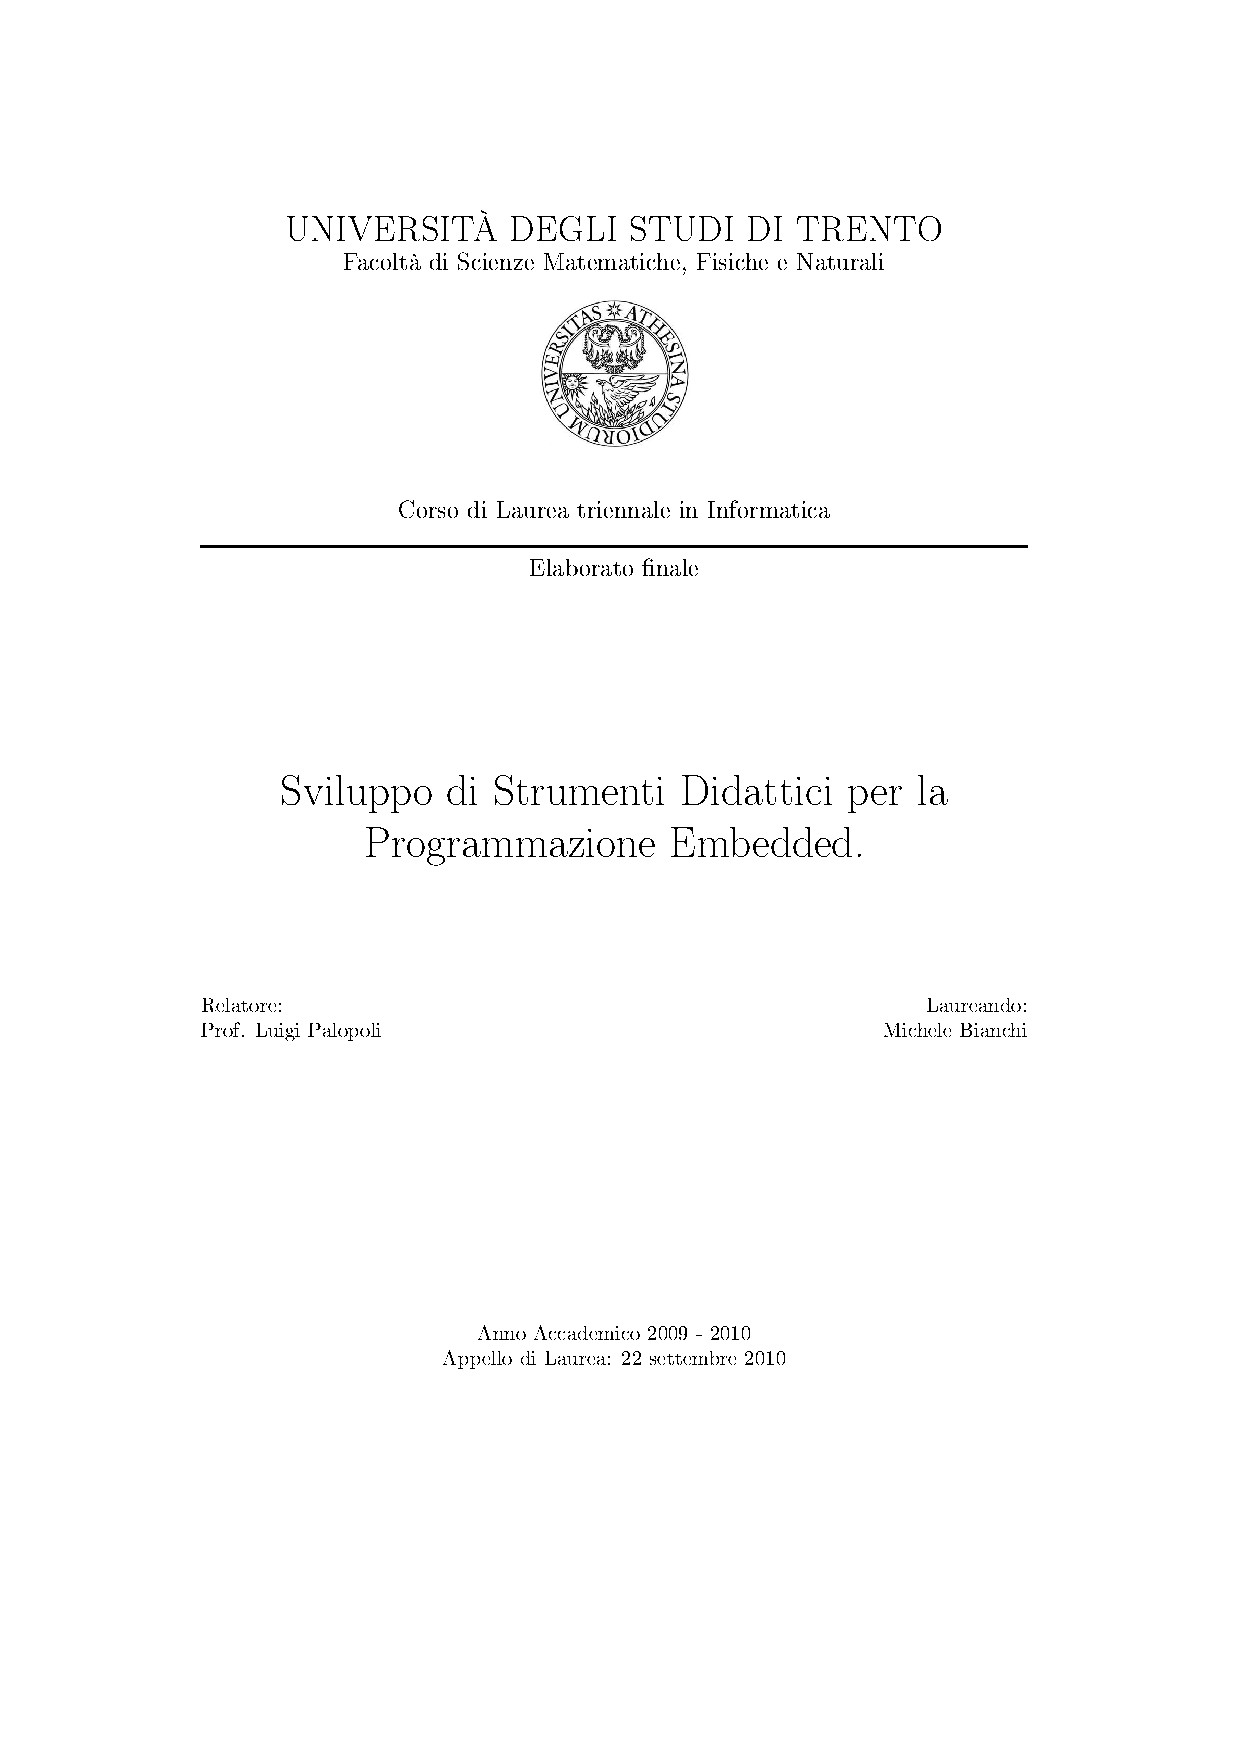
\includepdf[pages=1]{Official/cover.pdf}

    \tableofcontents
    \cleardoublepage
    
    \chapter*{Ringraziamenti e Roba Varia}
\label{chap:Thanks}

\emph{Venerdì 17 Settembre 2010, Ore 19:00. Aula Studio del Padiglione 3
dell'FBK}

Anche se questo è il primo capitolo (anzi, addirittura direi che è lo
zeresimo o il ``menounesimo'') sappiate che è l'ultimo. Perchè? Boh.
Probabilmente volevo godermelo, perchè non volevo essere troppo di fretta
nello scriverlo.

\'E stata una dura lotta. Sono quasi sette mesi che lavoro dietro a questo
progetto. Ne ho passate di strane. Ho visto cose che speravo non avrei
visto. Ho provato cose alle quali pensavo di essere immune. Ho imparato
molto, cosa che mi ha dimostrato di quanto ero scarso all'inizio. Prima
pensavo di saper programmare. In realtà sapevo solo... Fare dello
\foreignword{scripting}. Adesso, grazie a questo progetto e anche grazie
all'esame \techname{Architettura degli Elaboratori} del mio relatore, il
professor \emph{Luigi Palopoli}, le mie viste si sono espanse. Come lo sono
le mie competenze tecniche.

Questo, ovviamente, non è stato solo grazie a me. Se non fosse stato per la
presenza e per l'aiuto datomi da certe persone sarei ancora là a bazzicare
tra le mie incertezze e le mie ``competenze'' incompetenti.

In questo tempo, inoltre, ho passato dei momenti assurdi. Se devo essere
sincero, per quanto mi siano parsi negativi, sono stati degli ottimi
momenti. Dovete capire che per me ogni momento che lascia qualcosa dentro è
un momento positivo. 

Ho passato una settimana dove pensavo di morire. Realmente. Andavo a letto
e tutto quello che riuscivo a pensare era che, probabilmente, il mio cuore
si sarebbe fermato durante la notte. Il giorno dopo, invece, avevo paura
di non riuscire ad arrivare a questo momento.

Durante un altro periodo dormivo quattro ore a notte. L'insonnia, sapete.
Dopo qualche giorno che si soffre d'insonnia le giornate sono accompagnate
da dei rari istanti dove la mente vaga e si perdono dei minuti dove,
magari, la gente ti ha detto qualcosa e non hai sentito. Oppure ancora
arrivano delle momentanee allucinazioni dove ti sembra di finire da un
piano all'altro, andare a sbattere contro le scale presenti dall'altra
parte della rampa che stai percorrendo, per poi accorgerti che sei fermo.

Tutti questi momenti, però, mi hanno dimostrato una cosa. Sono tutte
stupidaggini. Il nervosismo. Meh. Infatti eccomi quì. Ciò che non uccide
rafforza, giusto? Inoltre tutto questo mi ha dimostrato che per me è
possibile farlo. Arrivare in fondo ad un impegno così importante. Ho
passato un anno dove non ero assolutamente convinto, dove non vedevo la
fine.

\'E stato alla fine di quell'anno, dopo un periodo orribile, dove ho
camminato solo la sera di Natale da Ravina a Trento, che ho visto come
andava affrontata la vita, almeno la mia\footnote{Anche perchè non sono quì
per scrivere un libro da motivatore fallito. Se ne volete uno potete andare
in libreria. Ci sono già troppi motivatori con la loro filosofia da
Americani che riempiono la nostra testa di cose inutili.}.

Ed è stato così che lì, nella mia mente, c'è un qualcosa che mi spinge
avanti. Un obiettivo che mi permette di affrontare gli esami che non
comprendo, un motore che, per citare qualcosa a me caro\footnote{E anche a
molti di quelli che mi hanno seguito in questa epica Quest}, mi permette di
``fare l'impossibile, vedere l'impossibile [...] toccare l'intoccabile'' e
di focalizzare la mia forza di volontà, per quanto facilmente distraibile.

Ed è così che sono arrivato quì. Grazie a questo e grazie a tutte quelle
persone che sono state con me fino in fondo. O che, semplicemnte, hanno
bazzicato dalle mie parti anche per poco tempo.

\section*{Ringraziamenti}
Intanto vorrei dire una cosa a tutti. Scusatemi. \'E stata una cosa dura e
la mia mente era preparata a questo solo fino ad un certo punto. All'inizio
l'impatto è stato quello che è stato. Quando è iniziata l'esate, però, ho
iniziato a notare una cosa. La mia soglia dell'attenzione ha incominciato a
calare vertiginosamente. Quando non lavoravo alla tesi lasciavo vagare la
mente, probabilmente ignorando alcuni dei vostri discorsi.

Inoltre la mia soglia di sopportabilità è calata. Penso di aver trattato
male della gente che non se lo meritava, di aver ignorato altri. Anche se,
penso, probabilmente con alcuni ho anche trovato in questa situazione la
forma mentis per comportarmi come dovevo.

Comunque chi è importante per me comunque è stata riposta nella mia mente
piena di milioni e milioni d'insulti e di nervosismi in una zona a contatto
limitato con essi, perciò sono salvi. Vi voglio bene, ragazzi. \'E sempre
dura dirlo, ma adesso sono abbastanza calmo per esserne convinto.

Vorrei comunque fare una lista di persone che meritano delle
menzioni\footnote{Oh, suvvia, se non siete presenti in questa lista non
vuol dire che vi odio.}

Inizierei col ringraziare due persone che, probabilmente, stanno leggendo
questo testo e si stanno chiedendo \emph{``Ma perchè non può semplicemente
evitare?''}. Probabilmente pensavano anche che mi sarei dimenticato di
loro, ma come potrei? Anche se sono spesso fuori sono sempre là. E non
pensiate che non mi senta in colpa per il tempo extra che ci ho messo.
Grazie dunque ad Enzo ed a Luisa, i quali mi sopportano ogni giorno
dell'anno.

Un altro ringraziamento, ovviamente, va al professor Luigi Palopoli, il
quale si è trovato una persona che arriva in ritardo, che si dimentica
degli appuntamenti e che gli presenta dei prototipi in \techname{Python}.

Ed ora iniziamo con una lista lunghissima 

\section*{SPAM: Origine di un nome}
\image  {Pictures/SPAM}
        {Un'immagine dello \SPAM{} nella sua ultima versione,
            sviluppata dal Maestro Ivan ``GODS'' Simonini.}
        {.8}
        {img:spam}
In giro per il testo potrei aver utilizzato il nome \SPAM{}. Devo ammettere
che questa scelta potrebbe creare della confusione nei lettori. Ma non vi
preoccupate, ora spiegher\'o in maniera abbastanza rapida cosa significa,
che cosa \'e e tutto il resto.

\cleardoublepage

    
    \part{Introduzione e Nozioni di base}
    \chapter{Introduzione}
\label{chap:Intro}

\section{I Sistemi Embedded}

\graffito{I Sistemi Embedded nella vita di tutti i giorni}
Negli ultimi tempi le vere rivoluzioni tecnologiche si sono sempre
dimostrate quelle riguardanti l'integrazione di device nella vita di tutti
i giorni senza che le persone che ne usufruiscono si accorgano della loro
presenza. Basta pensare alla enorme quantit\'a di device con la quale
siamo abituati a convivere, quali navigatori satellitari che stanno nel
palmo della mano, integrati all'interno degli smartphone, ormai
potenti quanto PC, oppure alla presenza di sistemi di controllo
elettronici per la stabilit\'a all'interno delle macchine.

Questi oggetti fanno parte di una categoria di sistemi
microprogrammati, noti come \newterm{Sistemi Embedded}, creati per eseguire
un numero limitato di specifiche funzioni. L'applicazione di questa
tecnologia spazia dalla robotica all'Entertainment portatile, dalla
medicina alle applicazioni militare, dunque si fa sempre pi\'u
necessario avere competenze
in questo campo, in quanto la richiesta \'e destinata ad aumentare,
come aumenter\'a la necessit\'a di avere strumentazioni tecnologiche sempre
pi\'u integrate nella vita di tutti i giorni, senza che l'utente finale si
accorga della loro presenza.

\section{Programmare i Sistemi Embedded}

Programmare applicazioni per questi sistemi pu\'o essere
estremamente complicato, soprattutto per coloro che sono meno esperti nella
programmazione o che sono abituati a produrre software per piattaforme di
alto livello.

\graffito{Le difficolt\'a derivanti dalla programmazione di software per sistemi
Embedded} Il problema derivante dalla programmazione di software per
sistemi Embedded \'e la necessit\'a di lavorare con risorse limitate.
Questo limita il livello di astrazione dei linguaggi di programmazione:
il programmatore necessita di competenze specifiche in linguaggi di basso
livello.
Il debugging di questo tipo di piattaforme, inoltre, pu\'o essere
complicato o impossibile: potrebbero non essere disponibili
periferiche di comunicazione diretta oppure metodi per
recuperare file di log direttamente dalla memoria del sistema.

Sviluppare le abilit\`a necessarie per programmare correttamente su questo
tipo di piattaforme pu\`o richiedere molto tempo. Per questo motivo \`e
utile disporre di una piattaforma di sviluppo sulla quale la
programmazione risulti pi\`u astratta e semplice, a cui venga demandata la
generazione dell'effettivo codice a basso livello. Tale approccio porta
due principali benefici:

\begin{itemize}

\item   Permette all'utente di sviluppare software pur senza richiedere
        competenze in programmazione;

\item   Costituisce una base di partenza per un programmatore inesperto
        che intraprende uno studio nel campo della programmazione
        Embedded.

\end{itemize}

\graffito{L'idea alla base}
L'idea \`e dunque quella di creare un set di strumenti che permettano di
spostare
lo sviluppo di software su un'applicazione di modellazione e simulazione
di sistemi dinamici, pur mantenendo un feedback istantaneo da parte della
piattaforma hardware.

Questo differisce dal metodo tradizionale di modellazione: nel caso di un
robot, per esempio, questo permette l'utilizzo di dati influenzati da
fattori esterni, quali la carica della batteria dell'unit\'a, l'attrito
intrinseco dei singoli motori, la presenza di ostacoli e cos\'i via.
Un software sviluppato in questo modo fa riferimento a \foreignword{real
case scenarios}.

In un ambiente di sviluppo tradizionale, al contrario, \`e necessario
introdurre degli elementi esterni ``fittizi'', oppure scrivere il codice
relativo al modello creato, testarlo sulla piattaforma Embedded,
registrare i dati per una seconda analisi e modificare il modello fino a
convergere ad una versione definitiva.

\section{Scelta degli strumenti}

In tutti i campi di applicazione delle Scienze Informatiche, la scelta di
strumenti di sviluppo corretti \'e un punto particolarmente cruciale.
In ambito Embedded questo riguarda non solo la piattaforma
\foreignword{software}, ma anche quella \foreignword{hardware}. Nel nostro
caso un'ulteriore opzione riguarda il \emph{pacchetto di modellazione e
simulazione di sistemi dinamici}.

Una volta effettuate tutte queste scelte, sar\`a necessario sviluppare un
sistema di interfacciamento della piattaforma Embedded con il software
di simulazione.

\subsection{La piattaforma Hardware}

Per quanto riguarda l'hardware \`e stato necessario individuare la
piattaforma che facilita maggiormente l'acquisizione di competenze
basilari nella programmazione Embedded.

Come accennato precedentemente l'idea che sta alla base dei sistemi
Embedded \'e la focalizzazione delle piattaforme hardware su un compito
specifico, tuttavia progettare specificatamente una piattaforma per lo
scopo prefissato sarebbe una spesa eccessiva.

\subsubsection{\nxt}

La scelta pi\`u naturale, seguendo criteri di basso costo e ampia
disponibilit\`a, \`e ricaduta sui \nxt.

Questa linea di prodotti della \lego \`e stata ideata per la costruzione di
robot e altri sistemi automatici o interattivi. \graffito{ATMEL
AT91SAM7S256} I \nxt{} contengono un \foreignword{microcontroller
multi-purpose} \techname{ATMEL} \techname{AT91SAM7S256}, piattaforma che
dispone di:

\begin{itemize}
\item Connessione \techname{USB};
\item Controller Bluetooth;
\item \foreignword{Bus} \isquarec per la comunicazione interna;
\item Connessione seriale \techname{RS485} (utilizzabile, tra gli altri
      possibili scopi, per la comunicazione tra \nxt).
\end{itemize}

La piattaforma \techname{AT91SAM7S256} \'e basata su un processore
\techname{ARM7}. Oltre ad essere facilmente reperibile, essa \`e stata e
viene tutt'ora utilizzata in vari prodotti distribuzione, quali:
\graffito{L'uso del processore ARM7 sul mercato}
\begin{itemize}
    \item \techname{Sega Dreamcast}
    \item \techname{Apple iPod}
    \item \techname{Nintendo DS} e \techname{Nintendo GBA}
    \item La maggior parte dei telefoni portatili della \emph{Nokia}
    \item Una gran quantit\'a di modelli di automobili.
\end{itemize}

Inoltre i \nxt{} vengono spesso utilizzati per scopi didattici in scuole 
e musei di scienze. In questi ambiti \`e molto popolare l'interfaccia di
programmazione visuale fornita di serie dalla \lego, la quale per\`o
risulta completamente inadeguata allo sviluppo di qualsivoglia programma
non banale.

\subsubsection{Periferiche disponibili per l'NXT}

Un altro punto forte dei \nxt{} \'e la disponibilit\'a di una vasta gamma
di sensori, inclusi nella confezione base, con i quali il software \`e in
grado di interagire con il mondo esterno:

\begin{itemize}
\item   Sensori di contatto binari;
\item   Sensori di luminosi\`a;
\item   Sensori acustici;
\item   Dispositivo \foreignword{sonar} a ultrasuoni;
\end{itemize}

\subsection{La piattaforma Software}

Una volta deciso su quale piattaforma hardware operare, occorre selezione
una delle varie varie alternative tra le molte piattaforme software
disponibili.

Le scelte vagliate sono state fondamentalmente tre:
\begin{description}
    \item[nxOS]\cite{bib:nxos} un sistema operativo per \nxt{} scritto da
    David Anderson. Purtroppo lo sviluppo comunitario di tale sistema
    appare abbandonato dal giugno del 2009.
    \item[NBC \& NXC]\cite{bib:nbcnxc} due firmware implementanti
    rispettivamente un linguaggio \techname{Assembly-like} ed un dialetto
    del \techname{C}.
    \item[nxtOSEK] un sistema operativo conforme allo standard
    \techname{OSEK} \cite{bib:osek} e sviluppato da Takashi Chikamasa.
\end{description}

Da questo punto di vista un ottimo indice di bont\`a \`e l'affidabilit\`a
dei \foreignword{device drivers} di sensori e servomotori: dopo svariati
test effettuati su queste piattaforme software, la scelta \'e ricaduta sul
sistema \techname{nxtOSEK}.

\subsubsection{Il sistema \nxtOSEK}

Il sistema operativo \nxtOSEK{}\cite{bib:nxtosek} \`e costituito
dall'unione dei device drivers in C/Assembly di \techname{LeJOS NXJ} (un
firmware di rimpiazzo per i \nxt{} basato su \techname{Java}) con il core
\techname{Toppers}.

\begin{description}
    \item[TOPPERS/ATK](conosciuto anche come \techname{TOPPERS/OSEK}), 
        fornisce primitive di \foreignword{multithreading real-time}
        conforme alla specifica \techname{OSEK};
    \item[TOPPERS/JSP]fornisce primitive analoghe conformi con le
        specifiche giapponesi \emph{$\mu$ITRON}\cite{bib:muitron}.
\end{description}

Grazie all'unione di queste features e all'utilizzo di una
\foreignword{toolchain} \techname{GCC} per \techname{ARM},
\techname{nxtOSEK} fornisce un ambiente di sviluppo Real Time in Ansi
\techname{C / C++}.

Per quanto funzionante, questo sistema operativo \`e tutt'altro che
perfetto, ma si rivela essere comunque la miglior scelta tra quelli
disponibili: i linguaggi supportati sono diffusi e ben conosciuti tra i
professionisti, dunque non \`e necessario un \foreignword{training}
specifico per sviluppare applicazioni. In pi\`u, fatta eccezione per parte
del sistema di compilazione, il sistema \`e completamente
\foreignword{Open Source}.

\subsection{Ambiente di Sviluppo Grafico}

Come menzionato precedentemente, la programmazione di basso livello su
piattaforme Embedded \'e complicata e, soprattutto, richiede un gran
numero di \foreignword{trial and error} con un \foreignword{feedback}
minimo da parte della piattaforma. Per questo motivo risultano
apprezzabili sia un sistema semplice ed intuitivo per la realizzazione di
applicazioni che un meccanismo per il logging di ci\'o che accade
sull'unit\'a NXT.

\subsubsection{Uno strumento di Modellazione e Simulazione}

In molti contesti di ricerca, la simulazione e la progettazione di
sistemi Embedded viene affidata al software \techname{Matlab}, un ambiente
per la computazione numerica. Questo viene in genere affiancato a
\techname{Simulink}, un pacchetto per la modellazione e la simulazione di
sistemi Dinamici ed Embedded.

Questo connubio permette ai professionisti della modellizzazione teorica di
sistemi elettronici di creare dei modelli per piattaforme Embedded, che
vengono successivamente testati senza dover scrivere il codice. Ci\`o
elimina la necessit\'a di competenze in programmazione.

\graffito{L'uso di \techname{SciCosLab}}
Sfortunatamente \techname{Matlab} viene distribuito a pagamento e con
licenza proprietaria, caratteristiche che non sempre sono accettabili in
un contesto accademico. In linea con il resto del progetto, esiste
comunque un'alternativa \foreignword{OpenSource} a \techname{Matlab} e
\techname{Simulink}, che rispettivamente possono essere sostituiti da
\techname{SciLab} e \techname{SciCosLab}.

\section{Implementazione}

Come a questo punto risulter\`a lampante, il lavoro descritto in questo
documento \`e stato incentrato sull'estensione del sistema
\techname{SciCosLab}, finalizzata all'inserimento di funzionalit\`a di
controllo remoto e raccolta dati sulla piattaforma Embedded \nxt.

Prima di inoltrarci nei dettagli tecnici dei capitoli successivi,
introdurremo, in una veloce panoramica, i vari sottoproblemi che sono
stati affrontati prima di poter attuare l'estensione di cui sopra.

\subsection{Lettura dei dati}

In \nxtOSEK{} come negli altri sistemi operativi testati, la comunicazione
attraverso il canale \techname{USB} risulta possibile solo in scrittura
(da computer a NXT). Come diretta conseguenza, \`e possibile comunicare al
robot le operazioni da eseguire, ma non si possono ottenere i dati rilevati
dai sensori. Operazioni comuni come il \foreignword{fine tuning} degli
attuatori e \foreignword{debug} ne risultano estremamente penalizzate.

Per questa ragione si \`e reso necessario lo sviluppo di un protocollo di
trasmissione basato su \techname{BlueTooth} col quale ottenere una
comunicazione bidirezionale.

\graffito{BROFist}Questo protocollo incorpora un formato binario per la
specificazione di comandi per il controllo dei servo motori e dei sensori,
cos\'i da poter costituire un radiocomando basato su computer.

A questo protocollo ho dato il nome di \BROFist{}: BROFist - Robot
Operational Fist, che sta ad indicare il rapporto di fratellanza che si
crea tra Robot e Computer grazie al suo utilizzo.

\subsubsection{Il problema del controllo remoto via BlueTooth}

Bench\`e praticabile, la comunicazione via \techname{Bluetooth} soffre di
latenze che si aggirano sui $45ms$ dovute alla pessima implementazione del
\foreignword{device driver} (i cui dettagli saranno affrontati nel
Capitolo~\ref{chap:SPAMC}).

Una simile latenza di non sarebbe un problema se si volesse utilizzare
il sistema solo per il plotting o per il logging dei dati letti dai
sensori, ma \`e palesemente inadeguata in caso di implementazione di
\foreignword{PID Controller} o altri sistemi di controllo.

\subsection{Il BROFist Client per lo SPAM}\label{sec:BROClient}

Una delle parti importanti del progetto \'e stata la scrittura, lato NXT,
di un client per l'interpretazione dei \emph{BROFists}, oltre che di
controllo della velocit\'a dei motori.

\graffito{Struttura del BROFistClient}
Il client \'e formato da quattro \foreignword{task}, ognuno con il suo
compito specifico:

\begin{description}
    \item[Comunicazioni Bluetooth e Decodifica dei BROFists]utilizzando
        le definizioni per il protocollo condivise tra tutte le parti del
        progetto. Questo \'e, fondamentalmente, il nucleo dell'intero
        Client: recupera i dati richiesti dai vari sensori e setta le
        potenze o le velocit\'a da raggiungere per i singoli servomotori;
    \item[Calcolo delle velocit\'a istantanee dei motori]il quale legge
        periodicamente i dati dei sensori tachimetrici e li registra
        all'interno delle strutture contenenti i dati dei singoli
        servomotori;
    \item[Controllo della velocit\'a dei motori]tramite l'utilizzo di un
        \PID, il quale usa i dati relativi alle
        potenze ed agli errori di velocit\'a per calcolare quanta potenza
        utilizzare per far andare i motori alla velocit\'a richiesta.
    \item[Rappresentazione di dati sullo schermo]utilizzando un comando
        delle API di \nxtOSEK{}. Naturalmente questi dati possono venir
        configurati modificando il codice sorgente del client.
\end{description}

\cleardoublepage

    \chapter{Background}

In questo capitolo parleremo del background tecnico e culturale che sta
dietro a questo progetto. Ci sar\'a spazio per una breve storia dei \nxt{}, 
delle veloci nozioni riguardanti al \PID{} e del \emph{Bluetooth}.

\section{I MINDSTORMS e gli NXT}
I \nxt{} sono l'ultima incarnazione di una serie di prodotti creati
dalla \emph{Lego}, la quale affonda le sue radici da una serie di sensori
programmabili venduti prima del 1998 dalla \emph{Lego}.

\subsection{Storia dei Lego MINDSTORMS}
La prima versione
della serie si chiamava \RIS{} ed \'e stata rilasciata sul mercato nel
1998, seguita poi nel 2006 dalla versione \emph{MINDSTORMS NXT}. Nel 2009
\'e stata pubblicata l'ultima edizione, chiamata \emph{MINDSTORMS NXT 2.0}.

\graffito{Le origini, prima della \emph{Lego}}
La base hardware e software della prima versione dei \emph{Lego Mindstorms}
\'e derivata direttamente dal lavoro dell'\emph{MIT Media Lab}, i quali
avevano creato dei brick programmabili a scopo didattico. Questi erano stati 
programmati in \emph{Lego Logo} ed avevano un ambiente di sviluppo grafico
creato appositamente dalla \emph{Universit\'a del Colorado} nel 1994 con il
nome di \emph{LEGOSheets}.

\graffito{I vari contenuti dei kits dei \emph{Lego Mindstorms}}
Non tutte le versioni dei \emph{Lego Mindstorms} hanno avuto le stesse
dotazioni in campo di sensori e servo motori. La prima versione chiamata
\RIS{}, conteneva due motori, due sensori di tocco ed un
sensore di luce. La versione \emph{NXT} conteneva, invece, due \emph{Servo}
Motori, un sensore di luce, uno di tocco, uno sonoro ed uno di distanza.
L'ultima versione, infine, ha la stessa dotazione di quella precedente,
solo con due sensori di tocco invece di uno soltanto. 

\graffito{L'uso dei \emph{Lego Mindstorms} in campo didattico}
I \emph{Lego Mindstorms} sono derivati, come accennato sopra, da un applicazione 
di tipo didattico dell'\emph{MIT Media Lab}. Per questo la Lego ha deciso
di continuare a seguire questa idea proponendo alle scuole dei set
didattici chiamati \emph{Lego Mindstorms for Schools}. Questi set,
conosciuti anche come ``Challenge set'', differiscono da quelli in
commercio normalmente per un sensore di luce extra, alcuni ingranaggi in
pi\'u ed un software per la programmazione dei brick differente.

Questo software, chiamato ``ROBOLAB'', \'e basato sul software ``LabVIEW''
della \emph{National Instruments}, un ambiente di sviluppo per il
loro linguaggio di programmazione visivo per l'automatizzazione
industriale. Un altra scleta per la programmazione dei bricks \'e
l'utilizzo di firmware o linguaggi di programmazione di terze parti, tra i
quali anche linguaggi conosciuti come il \emph{C} o il \emph{JAVA}, i quali
vengono usati dai professionisti in campo di programmazione embedded.

\subsubsection{L'origine del nome \emph{Mindstorms}}
I \emph{Lego Mindstorms} devono il loro nome al titolo del libro
``Mindstorms: Children, Computers, and Powerful Ideas'', scritto da \emph{Seymour
Papert}, uno dei pionieri dell'Intelligenza Artificiale ed inventore del
\emph{LOGO}. In questo libro Papert proponeva un ambiente di studio basato
sui computer chiamato \emph{il Micromondo}.

Questo Micromondo doveva completare il metodo di costruzione della
conoscenza dei bambini, conosciuto come \emph{Approccio Costruttivista
all'insegnamento ed al sapere}.

Siccome i \emph{Lego Mindstorms} hanno alla base proprio questa idea
perci\'o la \emph{Lego} ha deciso di utilizzare questo nome.

\section{Lego MINDSTORMS - RCX}
La prima versione dei \emph{Lego Mindstorms} aveva come base il brick
conosciuto come \emph{RCX}.
\graffito{Specifiche tecniche dell'RCX}Contiene un microcontroller 
\emph{Renesas H8/300} come CPU ed una memoria RAM di 32KB. L'unica
interfaccia di comunicazione con il PC o gli altri RCX \'e una porta
\emph{InfraRed} (IR). Questo rende impossibile l'upload di programmi
sull'RCX con metodi differenti da un'interfaccia proprietaria IR per la
quale esistono drivers solo per Windows e MAC. \'E possibile caricare
programmi anche in ambiente \emph{*NIX}, utilizzando per\'o metodi
differenti, quali il compilatore per \emph{Not Quite C}.

Oltre alla porta IR sono presenti tre porte per i sensori, tre per i
motori ed un LCD sul quale si poteva leggere la carica della batteria, lo
stato di motori e sensori, il programma in esecuzione oppure quale
programma era in esecuzione al momento.

I programmi, sull'RCX, vengono mantenuti sulla memoria RAM, quindi ogni
volta che veniva spento il brick questi vengono cancellati ed vanno
ricaricati sul brick. Questo problema, nella versione 1.0 degli RCX, \'e
risolto grazie alla presenza di un jack per la connessione ad un
caricatore.


\cleardoublepage


    \part{Sviluppo di BROFist}
    \chapter{Il Client di BROFist per SPAM}
\label{chap:SPAMC}

In questo capitolo parleremo dello svilupppo del client per \SPAM{} del
progetto \BROFist{}, dei problemi riscontrati e dei test effettuati per
limitarne l'impatto.

\section{Creazione di SPAM}
Il robot sul quale è stato creato l'intero progetto non è sempre stato
nella forma attuale. All'inizio il modello utilizzato era quello proposto
dalla \emph{Lego} nelle istruzioni base contenute nelle scatole dei
\nxt{} (Si faccia riferimento all'immagine \ref{img:orignxt}).
\image  {Pictures/StandardNXT}
        {Una delle versioni base di un \nxt{}, costruita seguendo le
        istruzioni contenute nei kit forniti dalla lego}
        {.5}
        {img:orignxt}

\graffito{Il problema di usare il modello presentato dalla \emph{Lego}} 
Dopo poco, però, anche grazie all'aiuto di Ivan Simonini, si è capito che
quella struttura aumentava gli errori di rotazione dei motori a causa di come era
stato pensato.

I motori erano montati in maniera tale che tutto il peso dell'unità
gravasse a metà tra i due, dove non era presente nessun punto di scarico
delle forze. Questo portava ad un'inclinazione verso il centro delle ruote,
facendo sì che non si muovessero in linea retta, richiedendo l'uso di un
feedback controller.

Viste le premesse è stato richiesto ad Ivan Simonini, che al tempo lavorava
come esperto presso il museo di scienze naturali di Trento, di controllare
l'unità e di renderla più strutturalmente stabile.

Il processo ha richiesto un mese e due prototipi, anche a causa della
scarsità di parti presenti nelle scatole \emph{Educational} dei \nxt{} e
delle richieste iniziali per il progetto, ovvero avere la possibilità di
montare un sensore di distanza brandeggiabile parallelo al terreno ed un
sensore di luce puntato verso il terreno a circa un centimetro da esso.
\graffito{La necessità di avere il sensore parallelo al terreno}
Il sensore di distanza doveva venir necessariamente montato in maniera
parallela rispetto al terreno in quanto il sistema di rilevamento della
distanza funziona con l'utilizzo di ultrasuoni. Questi vengono emessi dal
sensore il quale, misurando dopo quanto tempo ritorna l'onda, calcola la
distanza dall'ostacolo puntato (Fare riferimento all'immagine
\ref{img:sonarpr}).
\image  {Images/SonarPrinciple}
        {Teoria base del Sonar Attivo, utilizzata dai sensore di distanza
        ad ultrasuoni per \nxt{}}
        {1}
        {img:sonarpr}

Questo sistema, però, è influenzato dall'angolazione della superficie
rispetto all'origine dell'onda, in quanto, se questa non è perpendicolare o
di pochi gradi differente rispetto all'angolo retto, l'onda 
rimbalza in una direzione differente da quella d'origine. Questo fa in
modo che non torni al sensore, il quale pensa di non aver alcun ostacolo di
fronte a se, oppure di averlo più lontano di quanto non lo sia realmente.

Proprio a causa di questo problema si fa necessario il montaggio dei
sensori in posizione parallela rispetto al terreno per eliminare almeno un
fattore di errore per la lettura della distanza.

Alla fine del processo di sviluppo e creazione, comunque, è stata costruita
l'unità \SPAM{} (Foto \ref{img:spam}), la quale ha un sensore di distanza
brandeggiabile parallelo al terreno, un sensore di luce e l'accesso diretto
al brick \emph{NXT}.

\section{Struttura e funzionamento del Client}\label{sec:clientstru}
Come già detto in precedenza (sezione \ref{sec:BROClient}) il client
\BROFist{} gira su un sistema \nxtOSEK{}, il quale fornisce tutte le
funzionalità real time necessarie all'esecuzione con deadlines richieste da
questo tipo di progetto. Il client è formato da quattro Task, i quali
collaborano per il controllo dello \SPAM{} e per la comunicazione con il PC.

Per ricapitolare i quattro Task hanno le seguenti mansioni:
\begin{itemize}
    \item Comunicazioni Bluetooth ed interpretazione dei
        BROFists (\ref{sec:BROCommS})
    \item Calcolo delle velocità istantanee dei motori (\ref{sec:BROSpdS})
    \item Calcolo ed attuazione delle potenze dei singoli
        motori (\ref{sec:BROPIDS})
    \item Output di dati sul Display LCD (\ref{sec:BROLCDS})
\end{itemize}

Vediamo rapidamente in dettaglio ogni Task, con alcuni dati tecnici, per
avere un'idea più chiara di quello che fanno:

\subsection[Task ``BRO\_Comm'']{Task ``BRO\_Comm'': Comunicazioni BT ed
interpretazione dei BROFists}\label{sec:BROCommS} 
Questo task è, fondamentalmente, il cuore di tutto il client. \'E
incaricato di comunicare via BlueTooth con il server, ricevere i dati,
interpretarli, far fare allo \SPAM{} ciò che è stato richiesto e quindi
mandare un'eventuale risposta al server.

Per fare questo è stato necessario un lungo periodo di ricerche e test per
comprendere come funzionino le API per la gestione delle comunicazioni
BlueTooth ed avere ben in mente come fosse strutturato il protocollo di
comunicazione \BROFist{}, cose delle quali parleremo nelle sezioni
\ref{sec:BROTooth} e \ref{sec:theProtocol}.

Dopo aver superato gli ostacoli imposti dai device drivers (e dal
controller BlueTooth in se) lo svilupppo ha portato alla scrittura di un
Task con un'esecuzione ciclica ogni \cypher{2ms}, il quale recupera sette
\emph{BROFists} contemporaneamente quando sono presenti all'interno del
buffer del controller BlueTooth e quindi li interpreta.

\graffito{Perchè sette \emph{BROFists}}
La scelta di inviare sette \emph{BROFists} alla volta è data dal fatto che
sono presenti solo sette porte per la connessione di motori o sensori,
quindi l'idea è che le richieste non dovrebbero essere superiori a
quel numero. \'E anche vero che le persone potrebbero richiedere due dati
differenti dallo stesso Servo Motore, però si è considerato che un
programmatore possa derivare uno dei due valori avendo il primo.

\graffito{L'uso dei dati ricevuti}
Quando le richieste riguardano l'invio del dato letto da un sensore non ci
sono problemi nella gestione dei dati: i dati vengono letti dai sensori e
quindi vengono inseriti all'interno della struttura che andrà inviata al
server presente sul PC. Se viene inviato un valore di potenza o velocità
per i motori, invece, viene o chiamata la funzione per il calcolo della
potenza in base alla velocità oppure settato il primo valore all'interno
dell'array contenenti le potenze dei motori\footnote{Si faccia riferimento
alla sezione \ref{sec:BROStruct} per avere più informazioni riguardo alla
conformazione della struttura dei dati per il controllo dei motori}.

\graffito{I dati in uscita}
Una volta interpretati tutti i \emph{BROFists} il client forma una serie di
\emph{BROFists} di risposta, i quali contengono la richiesta ed il dato ad
essa correlato. Nel caso di potenza o velocità dei motori il dato è sempre
$0$.

\subsection[Task ``Speed\_Updater'']{Task ``Speed\_Updater'': Calcolo delle
velocità istantanee}\label{sec:BROSpdS}
La possibilità, da parte del server, di richiedere la velocità media di uno
dei servo motori e la presenza di un \PID{} ha reso necessaria l'aggiunta
di un Task per il monitoraggio e per l'aggiornamento dei dati riguardanti i
vari Servo Motori installati.

Il concetto di questo Task è molto semplice: ogni \cypher{5ms} viene letto i valori
dei Tachiometri presenti all'interno di ogni motore e vengono registrati
all'interno di un array circolare. Usando il valore precedente viene
calcolata la velocità istantanea di ogni valore e viene inserita
all'interno di un secondo array circolare.

Facendo ciò, dunque, avremo abbastanza dati per poter calcolare la velocità
media su \cypher{(5 * Dimensione dell'array circolare)ms}.

\subsubsection{Problemi derivanti dall'uso dei valori dei Tachiometri}
Il valore di ogni Tachiometro viene registrato all'interno di una variabile
di tipo \codeconst{int32_t}. Questo \emph{potrebbe} portare a dei problemi
dati dall'\emph{overflow} o dall'\emph{underflow} dato dall'eccessivo
utilizzo dei motori.

Questo, però, occorrerebbe soltanto dopo una rotazione continua, in una o
in un'altra direzione, di \cypher{$2^{31}$}°, ovvero
\cypher{2,147,483,648}°. Considerando il diametro delle ruote installate
sullo \SPAM{}, che sono quelle contenute nei Kit \techname{Educational} dei
\nxt{}, che misura \cypher{56mm} ed il fatto che esse sono collegate ai
Servo Motori tramite degli ingranaggi con un rapporto \cypher{1:1}, la
distanza che andrebbe percorsa da un singolo motore dovrebbe essere: $56mm
* 3.14 * (2,147,483,648 / 360)$, ovvero una distanza pari a $1,048,927m$.

\graffito{Un problema che non è un problema}
Questa distanza è fin troppo grande per venir considerata un problema,
visto che la carica della batteria e la velocità dei motori non
permetterebbero il raggiungimento di una cifra così grande.

\'E facile, comunque, che una frase simile si sia già sentita in passato nella
storia dell'informatica, portando a problemi e bug, ma la correzione di un
problema simile è facile e necessario solo in progetti che prevedono
l'utilizzo dei motori per una durata così lunga, perciò è stata lasciata in
dietro quasi volontariamente.

\subsubsection{Utilizzo di un array circolare per il calcolo della velocità}
Purtroppo la sensibilità dei Tachiometri integrati nei servo motori dei
\nxt{} è limitata ai gradi interi. Questo porta ad una propagazione
dell'errore di lettura quando si deve calcolare la velocità in
\cypher{Gradi al Secondo}, in quanto bisogna moltiplicare il valore
ricavato per una scala pari a \cypher{100 / Tempo di Sampling}.

A causa di questo, infatti, la sensibilità della velocità diventa, appunto,
pari alla scala che va applicata alla velocità per ogni intervallo di
Sampling.

Una sensibilità tale non è utile, in quanto inusabile dai vari algoritmi
di controllo\footnote{Anche perchè, in questa maniera, sarebbe obbligatorio
utilizzare come velocità target dei valori che sono dei multipli della
scala} visto che fanno uso dell'errore di velocità per ricavare la potenza da
applicare ai motori. Bisogna perciò trovare un altro metodo per il calcolo della
velocità media di un motore con i dati che ricaviamo dalla lettura
periodica dei Tachiometri.

\'E per questo che si è deciso di utilizzare una media mobile che usa le
ultime $10$ velocità istantanee.

\subsection[Task ``PID\_Controller'']{Task ``PID\_Controller'': Calcolo ed
attuazione delle potenze dei Motori}\label{sec:BROPIDS}
Siccome, anche a causa delle ``scarse''\footnote{Si faccia riferimento alla
sezione \ref{sec:BROTooth} per avere un'idea di questo problema}
prestazioni del BlueTooth sotto \nxtOSEK{}, non sappiamo esattamente quando 
saranno presenti dei nuovi dati per il controllo dei motori abbiamo bisogno
di un Task per il controllo periodico dei motori.

\'E per questo motivo che è stato implementato un Task periodico che, ogni
$5ms$, utilizza i dati per regolare la potenza dei vari motori.

Nel caso di controllo diretto delle potenze dei motori questo compito non è
particolarmente grave. Al Task, infatti, basta utilizzare l'ultimo valore
ricevuto come potenza da settare per il motore interessato.

\graffito{L'uso del \PID{}}
Quando, invece, viene richiesto di settare una determinata velocità il Task
deve far uso del \PID{}\footnote{Si faccia riferimento alla sezione
\ref{sec:PIDTheo} per un'idea migliore di cosa sia un \PID{}} implementato
tra le API del progetto.

Questo usa le ultime tre potenze utilizzate per il motore preso in
considerazione e le ultime tre differenze tra le velocità medie e la
velocità richiesta per calcolare la potenza da utilizzare per fare in modo
che i motori vadano alla velocità corretta. Una volta calcolato questo
valore lo utilizzano per far muovere i motori alla velocità richiesta
dall'utente.

\subsection[Task ``DisplayTask'']{Task ``DisplayTask'': Visualizzazione dei
dati sullo schermo LCD}\label{sec:BROLCDS}
Il compito di questo Task, eseguito ogni $1000ms$, è quello di fornire un
contatto con l'utente attraverso l'output di vari dati sull'LCD del Brick
dello \SPAM{}.

Questi dati sono configurabili, ovviamente, ma nella versione standard del
Client \BROFist{} i dati mostrati sono quelli raccolti dalla chiamata di
\nxtOSEK{} \codeconst{ecrobot\_status\_monitor(target\_name)}.

\subsection{Il Protocollo per \BROFist{}}\label{sec:theProtocol}
Per la comunicazione tra \SPAM{} e PC, ovviamente, si è resi necessari lo
studio e la realizzazione di un protocollo con il quale codificare le
richieste per lo \SPAM{}.

Per rendere questo lavoro più semplice è stato optato l'approccio più
facilmente implementabile in C, ovvero l'utilizzo di una struttura
contenente:
\graffito{Struttura di un \BROFist{}}
\begin{itemize}
    \item La codifica di quale sensore richiedere o di quale tipo di valore
        per il controllo dei motori è stato inviato. Per questa codifica si
        è deciso di utilizzare una variabile di tipo \codeconst{uint8_t},
        in quanto si è considerato che non esisteranno più di
        254\footnote{In quanto uno dei comandi dev'essere quello che
        dichiara finita la comunicazione} comandi
        differenti\footnote{Comunque la struttura del progetto è tale che,
        quando qualcuno deciderà di implementare più del massimo consentito
        da questo tipo di variabile, questo cambiamento sarà rapido e senza
        troppi problemi}
    \item La porta alla quale il sensore o servo motore è collegato. Anche
        questa codifica viene registrata all'interno di una variabile di
        tipo \codeconst{uint8_t}, vista la presenza di solo $7$ porte sul
        Brick \emph{NXT}.
    \item Il valore da settare in caso venisse inviata una richiesta di
        controllo di servo motori oppure il valore letto dal sensore
        richiesto. Per questo valore viene usata una variabile di tipo
        \codeconst{float}, in quanto la velocità richiesta potrebbe essere
        di tipo decimale, come la velocità media di un servo motore.
\end{itemize}

\graffito{Le codifiche delle richieste}
Al momento sono stati utilizzate le seguenti codifiche per le
richieste\footnote{Le quali sono definite, assieme a quelle per le porte,
all'interno del file header \cypher{broi\_fist.h} posto all'interno della
cartella \cypher{src/headers}}:
\begin{description}
    \item[LIGHT\_SENSOR] codificato come $1$, serve per la richiesta del
        valore letto da un sensore di luce
    \item[TOUCH\_SENSOR] codificato come $2$, serve per la richiesta del
        valore di un sensore di tocco
    \item[SOUND\_SENSOR] codificato come $3$, serve per la richiesta del
        valore registrato da un sensore di suono
    \item[RADAR\_SENSOR] codificato come $4$, serve per la richiesta della
        distanza letta da un sensore di distanza ad ultrasuoni
    \item[TACHO\_COUNT] codificato come $6$, serve per la richiesta del
        valore attuale del Tachimetro di un motore
    \item[AVG\_SPEED] codificato come $7$, serve per la richiesta della
        velocità media di un motore
    \item[SET\_SPEED] codificato come $8$, serve per inviare una velocità da
        settare ad un motore
    \item[SET\_POWER] codificato come $9$, serve per inviare una potenza
        ``grezza'' da settare ad un motore
\end{description}

Mentre le codifiche delle porte sono le seguenti:
\begin{description}
    \item[PORT\_1\textasciitilde{}4] codificate con i valori
        $1$\textasciitilde{}$4$, servono per applicare la richiesta ad una
        delle quattro porte per i sensori.
    \item[MOTOR\_A\textasciitilde{}C] codificate con i valori
        $5$\textasciitilde{}$7$, servono per applicare la richiesta ad una
        delle tre porte per i motori.
\end{description}

\section{BlueTooth e relativi problemi sullo SPAM}
I \nxt{} hanno due modi per comunicare con l'esterno: usando
l'\techname{USB} oppure il \techname{BlueTooth}. Nel progetto \BROFist{} si
è deciso di utilizzare la tecnologia \techname{BlueTooth} visto che il
progetto era puntato ad un utilizzo per la rilevazione telemetrica e per il
controllo realtime di un'unità \emph{NXT}, cosa che poteva risultare
complicata con la presenza costante di un cavo USB collegato all'unità.

Parleremo dunque prima della tecnologia in generale per poi spostarci ai
vari test che sono stati effettuati per calcolare la latenza delle
comunicazioni tra PC e \SPAM{} ed, infine, parleremo dei problemi
riscontrati nell'uso delle API di \nxtOSEK{} per l'uso del
\techname{BlueTooth}.

\subsection{Il BlueTooth}
Il \techname{BlueTooth} è uno standard Open per le comunicazioni a corto
raggio sviluppato dalla \emph{Ericsson} nel 1994. Questo permette la creazione di
\techname{Personal Area Network} ad alti livelli di sicurezza.

\graffito{Origine del nome BlueTooth}
Questa tecnologia deriva il suo nome dalla traduzione in inglese
dell'epiteto dato al re ``Aroldo I di Danimarca''. Il logo, invece, è la
runa derivata dall'unione delle rune che sono le iniziative del nome di
Aroldo: \textarn{h} e \textarn{b}.

\graffito{Funzionamento del BlueTooth}
Il \techname{Bluetooth} funziona tramite l'utilizzo di una tecnologia radio
chiamata \emph{Frequency-Hopping Spread Spectrum}. Questa tecnologia
suddivide i dati che vanno inviati e li trasmette su un numero massimo di
79 bande da $1$MHz l'una, tutte comprese nel range da $2402$ a $2480$MHz.

Il \techname{BlueTooh} utilizza un protocollo di comunicazione a pacchetti
con una struttura \emph{Master-Slave}, la quale permette la presenza di un
\emph{Master} e fino a $7$ \emph{Slaves} all'interno della stessa
\emph{picoNet}. Lo scambio di pacchetti viene regolato sul clock base,
regolato dal Master, il quale ha un intervallo di $312.5\mu{}s$. Il Master
utilizza gli slot per la comunicazione in maniera alternata: invia negli
slot pari e riceve in quelli dispari. I vari client, al contrario, ricevono
durante gli slot pari ed inviano in quelli dispari.

Questa struttura permette una comunicazione a corto raggio con un basso
consumo energetico. Il raggio di comunicazione è dato dalla classe del
device Bluetooth, andando da $1$m fino a $100$m.

La velocità massima di trasferimento è, nella maggior parte dei casi, di
$24$Mbit/s.

\subsection{La latenza della comunicazione BlueTooth tra PC ed
NXT}\label{sec:BROTooth} 
Prima di sviluppare completamente il sistema bisognava essere sicuri di
quanto tempo trascorresse tra l'invio di un \BROFist{} e la ricezione della
risposta, oltre al numero di errori di trasmissioni.

Per questo sono stati fatti un gran numero di test, prima solo in
ricezione, poi sia in invio che in ricezione. Questi test prevedevano il
cambiare distanza tra PC e \SPAM{}, aumentare gradualmente il numero di
test oppure cambiare la dimensione dei pacchetti inviati.

\graffito{I test di comunicazione SPAM $\rightarrow$ PC}
La prima serie di test effettuati prevedeva la ricezione di pacchetti in
serie spediti direttamente dallo \SPAM{} senza invii da parte del PC per la
sincronizzazione. Dopo una serie di test si è notato che la velocità di
comunicazione si attestava intorno ai $2ms$ e che non c'erano perdite di
dati durante le comunicazioni.

\graffito{I test di comunicazione PC $\rightarrow$ SPAM $\rightarrow$ PC}
Una volta completati i test per la comunicazione unidirezionale è stato il
turno di quelli bidirezionali, i quali prevedevano una sincronizzazione tra
PC e \SPAM{}.

Durante la prima fase dei test, eseguiti a varie distanze, tutte tra $1$ e
$10$ metri, la latenza delle comunicazioni, eseguite $100000$ alla volta, si
attestava intorno ai $4ms$.

Una volta controllati gli errori di comunicazione, però, si è notato che i
pacchetti ricevuti erano tutti errati. Molti dati non arrivavano,
sostituiti da valori casuali, tipici di letture di settori di memoria
errati. Questo ha portato ad una serie di test per la comprensione di quale
fosse il problema, oltre che a delle lunghe sessioni di \emph{Bugfixing}.
Dopo quasi un'intera settimana di lavoro intensivo, più di $50$ versioni
differenti di Server e Client e del \emph{Retro-Engineering} del codice dei
Device drivers di \nxtOSEK{} si è finalmente capito quale fosse il
problema.

\graffito{Problemi del BlueTooth sotto \nxtOSEK{}}
Il problema risiede sia nei Device Drivers che nel Controller BlueTooth
dei \nxt{}. La parte di problema dei Device Driver parte dal fatto che, pur
essendo presente un \techname{DMA} sulla piattaforma Hardware, non vengano
utilizzati gli Interrupt per gestire le comunicazioni via BlueTooth.
Infatti la chiamata che legge i dati da BlueTooth altro non fa che
controllare se sono presenti dei dati nel Buffer del
Controller\footnote{Richiedendo queste informazioni niente di meno che al
\techname{DMA} stesso} e quindi copiarli solo se sono esattamente quanti
indicati nel primo byte di dati ricevuti\footnote{In realtà lo spazio
``riservato'' per questa informazione dovrebbe essere di 2 byte, il secondo
dei quali viene ignorato dalla chiamata. Inoltre bisogna passare, come
parametro della funzione di lettura dei dati, la quantità di dati da
leggere. Una ridondanza di dati quasi inutile.} Questo fa sì che sia
necessario l'utilizzo di un approccio di \emph{polling} non bloccante,
creando un Task ad esecuzione periodica.

Questo Task dovrà agire soltanto quando ci sarà una risposta affermativa da
parte della funzione di lettura dei dati. Il problema dato da questo
approccio è quello derivato dalla perdita di tempo in caso i dati si
rendano disponibili tra un'esecuzione del Task ed un'altra.

Il ritardo, però, è stato limitato dando al Task un periodo di $2ms$,
facendo in modo che non possa trascorrere più di $1ms$ tra la ricezione
completa e l'utilizzo dei dati.

Utilizzando questo metodo, dopo una lunga serie di test da $30000$
comunicazioni bidirezionali alla volta, ha portato la latenza a $45ms$, ma
il numero di errori è stato portato a $0$.

\graffito{I probabili problemi dati dal Controller BlueTooth}
Questo, dunque, ci porta ad un'altra considerazione: se il ritardo è al
massimo di $1ms$ vuol dire che l'errore è in un altro punto. Questo ci
porta all'idea che, probabilmente, le prestazioni del Controller BlueTooth
installato sui \nxt{} non siano ottime come si sperava. Questa, però, è una
congettura in quanto non c'è un modo sicuro per dimostrare questo fatto.

\section{Problemi di sviluppo}
Durante lo sviluppo del Client sullo \SPAM{} e anche durante il
conseguimento delle abilità necessarie per il suo sviluppo sotto
\nxtOSEK{} ci sono stati dei problemi che hanno portato ad un sensibile
rallentamento di queste attività.

Oltre al problema di dover creare l'immagine da caricare sull'\nxt{} ogni
volta e poi caricarla riavviando tutto il sistema, cosa che prendeva al
mimimo un minuto al ciclo di spegnimento, carica dell'immagine ed
esecuzione, l'impedimento più grande è stato quello della mancanza di un
debugger.

Ogni volta che si presentava un bug non c'era modo di capire da cosa fosse
dovuto se non con una lunghissima serie di test e di letture di dati sullo
schermo LCD. Inoltre neanche quest'ultimo metodo era sempre disponibile in
quanto quando avveniva un qualche problema di lettura dei dati dalla
memoria sullo schermo compariva il messaggio \cypher{DATA ABORT} e l'intera
unità si bloccava, rimuovendo qualunque messaggio che era stato scritto
sul Display.

\cleardoublepage

    \chapter{Il Server di BROFist per PC}
\label{chap:PCServ}

In questo capitolo parleremo dello sviluppo del Sever per PC
del progetto \BROFist{} e delle librerie utilizzate.

\section{La struttura di BROFist}
Il progetto \BROFist{} è formato da tre parti ben distinte tra di loro:

\begin{description}
    \item[Un Client su NXT]il quale deve ricevere degli ``ordini'' ed
        eseguirli per poi inviare al Server i risultati di questi ordini.
    \item[Un Server su PC]il quale riceve degli ordini per lo \SPAM{} da
        parte dell'interfaccia grafica ed invia questi ordini al client in
        esecuzione sull'unità.
        
        Una volta ricevuta la risposta dal Client questa viene inoltrata
        all'interfaccia.
    \item[Dei blocchi d'interfaccia per SciCos]i quali si collegano al
        server, grazie al quale possono comunicare con lo \SPAM{} ed
        utilizzare i dati ricevuti nelle simulazioni.
\end{description}

Questa schematizzazione, però, è frutto di una lunga progettazione, la
quale è stata necessaria per creare il sistema più flessibile possibile,
oltre ad oltrepassare delle limitazioni del pacchetto grafico di
simulazione e modellazione \techname{SciCosLab}.

\subsection{La struttura di BROFist nel tempo}
\graffito{La prima versione}
L'idea iniziale era di creare semplicemente un logger che inviava in
realtime vari dati calcolati dal software in esecuzione sullo \SPAM{}, i
quali venivano ricevuti da un server scritto in \techname{Python}.

Il problema di questa struttura, però, era la mancanza di flessibilità, in
quanto, ogni volta che venivano cambiati i dati inviati, bisognava cambiare
il codice del server. Questo perchè il metodo utilizzato per
l'interpretazione dei dati ricevuti via \techname{BlueTooth} prevedeva
l'utilizzo della funzione \codeconst{struct.unpack}, la quale richiede una
stringa che indica la struttura dei dati da interpretare.

\graffito{La decisione di sviluppare un protocollo}
Per risolvere questo problema si è quindi deciso di sviluppare un sistema
che facesse uso di un protocollo per la richiesta di dati dei sensori e per
il controllo da remoto dei motori.

Questo, però, richiedeva lo sviluppo di un sistema che, ricevute le
richieste, si comportasse in accorodo con esse. \'E per questo che il
sistema è passato da un'applicazione che inviava dati ad un PC ad un
modello \techname{Client-Server}.

Per creare il Server, dunque, si è deciso di utilizzare \techname{C} invece
che \techname{Python}, in quanto c'era bisogno di una gestione delle
strutture a basso livello e di prestazioni migliori\cite{bib:progbench}.

La scelta di passare a \techname{C}, però, ha richiesto del tempo per
arrivare alle competenze necessarie\footnote{La quale, però, che è stata
facilitata grazie alla documentazione presente online
\cite{bib:blueZdocs}}.

\graffito{L'idea di creare dei blocchi d'interfaccia per SciCosLab}
Vista la possibilità di comunicare via \techname{BlueTooth} utilizzando
\techname{C} invece di \techname{Python} si è reso automaticamente
disponibile lo sviluppo di blocchi di codice per \techname{SciCosLab}.
Questo ha reso necessario lo strutturare il progetto in modo che
funzionasse tra blocchi di \techname{SciCosLab} ed il Client su \SPAM{}.

Dunque l'idea iniziale era quella di sviluppare il progetto in direzione di
un modello \emph{Client-Server} tra \techname{SciCosLab} ed \techname{NXT}.
Purtoppo, però, il pacchetto di modellazione \techname{SciCos} integrato in
\techname{SciCosLab} manca della flessibilità necessaria\footnote{Si faccia
riferimento al paragrafo \ref{sec:whyitsucks} per capire meglio quali sono
i problemi derivanti dallo sviluppo di blocchi in \techname{C} per
\techname{SciCos}} per sviluppare questo progetto.

\graffito{Il modello SciCosLab - Server - SPAM Client}
\'E grazie a questa serie di tentativi e di modelli che si è arrivati
all'idea finale per il progetto \BROFist{}, la quale prevede l'utilizzo di
blocchi d'interfaccia per \techname{SciCosLab}, i quali comunicazno con un
server che gira sullo stesso computer\footnote{Anche se, grazie alla
struttura data al progetto, non è escluso che si possa utilizzare un server
in remoto}, connesso ad uno \SPAM{} via \techname{BlueTooth}.

Grazie al questa struttura, dunque, abbiamo un sistema flessibile che
permette la sua estensione in base alle necessità dell'utente.

\section{Le ragioni dello sviluppo di un Server}
Abbiamo già detto che una delle motivazioni per la scelta di un modello
basato su server era la poca flessibilità data dallo sviluppo di blocchi
per \techname{SciCos}. Ovviamente questo non è stato l'unico fattore che ha
portato alla scelta fatta.

Il punto forte di questo sistema è l'estensibilità data dall'uso dei
\techname{Socket UNIX} e dal fatto che il codice utilizzato per comunicare
con l'\techname{NXT} è separato dall'applicazione che la necessita. La
schematizzazione di questa struttura e delle possibili estensioni future è
rappresentata nell'immagine \ref{img:BROFistStruct}

\image  {Images/TheBROFistStructure}
        {La struttura del progetto \BROFist{}, con i possibili sviluppi
        futuri, segnati come delle linee viola tratteggiate}
        {.8}
        {img:BROFistStruct}

Questo permette, conoscendo le strutture utilizzate per la comunicazione,
di sviluppare applicazioni di qualunque tipo che sfruttano il server per
comunicare con un'unità \SPAM{}, controllarne i motori oppure ricevere dati
dei vari sensori.

\graffito{Esempio di applicazione alternativa per BROFist: Web Interface}
Mettiamo, ad esempio, di voler creare un esperimento sociale attreverso la
rete dove la gente può prenotare l'utilizzo di un'unità \SPAM{} alla quale
è stata aggiunta una Webcam. Questa unità è stata posta all'interno di uno
spazio chiuso con vari oggetti coi quali interagire, ostacoli ed altro.

Per sviluppare questo progetto sarebbe necessaria un'interfaccia Web la
quale si collega via remoto ad un server \BROFist{} il quale manderebbe i
pacchetti di ordini allo \SPAM{} e spedirebbe indietro i dati letti dai
sensori, oltre che alle immagini della Webcam\footnote{Anche se i dati
della Webcam verrebbero gestiti dall'interfaccia Web.}.

\graffito{Gli altri sviluppi resi possibili dall'uso di un server}
Oltre alla possibilità di creare applicazioni ``ad hoc'' che usano il
server \BROFist{} questo tipo modello ci permette anche di estendere i
metodi di connessione del server allo \SPAM{}.

Per ora il sistema comunica solo via \techname{BlueTooth} però uno dei
possibili sviluppi futuri\footnote{Per quanto sia complesso utilizzare
l'\techname{USB}, visto che il supporto LibUSB è stato rimosso da
\nxtOSEK{} dalla release del 2009} potrebbe essere l'abilitazione delle
comunicazioni via \techname{USB} con l'unità \techname{NXT}.

Inoltre altre aggiunte potrebbero venir applicate a Client e Server per
permettere la comunicazione dei contenuti di variabili ben definite, oppure
per il controllo delle periferiche collegate alla porta \techname{RS485}.

\section{Il funzionamento del server}
Il server è diviso in quattro moduli separati, ognuna con delle funzioni
ben specifiche. Le quattro parti separate sono:

\begin{description}
    \item[Controllo BlueTooth]che contiene tutte le funzioni per la
        connessione e la comunicazione attraverso \techname{BlueTooth}
    \item[Controllo Socket UNIX]che contiene tutte le funzioni per la
        gestione del server, la comunicazione via \techname{Socket UNIX} e
        la sua interazione con le comunicazioni \techname{BlueTooth}
    \item[Parsing delle Opzioni]che si occupa di fare il \emph{parsing}
        delle opzioni e quindi comportarsi di conseguenza.
    \item[Il Server BROFist]il quale utilizza i dati settati dal Parser per
        iniziare le comunicazioni, fare il forwarding dei dati e quindi
        bloccarsi quando riceve l'ordine di stop.
\end{description}

Vedremo ora le varie funzionalità di ogni modulo, parlando anche delle
strutture utilizzate.

\subsection[bro\_bt]{bro\_bt: Gestione BlueTooth}
In questo modulo sono contenute tutte le funzioni per la gestione del
\techname{BlueTooth} per il server di \BROFist{}. Sono inoltre contenute la
dichiarazione della struttura per l'identificazione dei device
\techname{BlueTooth} e le defines per la discovery e per la connessione dei
devices.

La scrittura di questo modulo, come quello del controllo delle
comunicazioni via \techname{Socket UNIX}, ha richiesto del tempo per
comprendere il funzionamento delle \emph{API} di \techname{BlueZ}, il
\emph{Protocol Stack} ufficiale per Linux.

Le funzioni di questo modulo sono:
\begin{itemize}
    \item \codeconst{size_t bro_bt_scan_devices (bro_bt_device_t *)}, la
        quale serve per la \emph{Discovery} dei device \techname{BlueTooth}
        in range, inserendoli all'interno di un array di strutture di tipo
        \codeconst{bro_bt_device_t}.

        Questo serve sia per stampare a video la lista di device, sia per
        collegarsi ad un device sapendo il suo nome.
    \item \codeconst{int bro_bt_connect_device (int *, bdaddr_t)}, funzione
        che serve a connettere un device, conoscendone il \emph{MAC
        Address}. L'indirizzo dev'essere passato sotto forma di codifica a
        $6$ bytes, come richiesto dalla libreria
        \techname{BlueZ}\footnote{Operazione che potrebbe risultare
        complicata. Fortunatamente \techname{BlueZ} fornisce anche la
        funzione \codeconst{int str2ba(const char *, bdaddr_t * )}, la
        quale converte un \emph{MAC Address} da formato stringa a formato a
        $6$ bytes.}.
        
        La connessione viene quindi legata ad un \emph{Socket
        Descriptor}, che verrà utilizzato dal programma per comunicare con
        lo \SPAM{}
    \item \codeconst{int bro_bt_client_fist (bro_fist_t *, bro_fist_t
        *,int)}, funzione che invia un set di \emph{BROFists} ed aspetta la
        risposta. Una volta ricevuti i dati dallo \SPAM{} la funzione
        riempie un set di \emph{BROFists} di egual misura di quelli
        inviati contenenti i dati richiesti.
    \item \codeconst{int bro_bt_close_connection{int}}, la quale chiude la
        comunicazione ed il socket descriptor ad essa collegato.
\end{itemize}

In questo modulo, inoltre, è presente la dichiarazione della struttura per
rappresentare un device \techname{BlueTooth} all'interno del progetto
\BROFist{}, la quale è rappresentata nel listato \ref{lst:BROToothS}

\begin{figure*}[htbp]
    \begin{lstlisting}[caption=BlueTooth Device Identification Structure,
                       label=lst:BROToothS]
typedef struct {
    /* Human Readable Name (As set on the Device). */
    char       name[248];      
    /* Mac address stored in a bdaddr_t variable */
    bdaddr_t   mac;             
} bro_bt_device_t;

    \end{lstlisting}
\end{figure*}

\subsection[bro\_comm]{bro\_comm: Gestione Comunicazioni via Socket UNIX}
Forse il modulo più importante del progetto, \emph{bro\_comm}, contiene le
funzioni per il controllo dell'\emph{IPC Socket} per la comunicazione con
le applicazioni sul PC, oltre che all'interazione tra \emph{IPC Socket} e
\emph{BlueTooth Socket}.

Le funzioni presenti in questo modulo sono solo tre:
\begin{itemize}
    \item \codeconst{int bro_start_server (int *, int *)} la quale
        inizializza il server, aspetta una connessione da un client che
        utilizza gli \emph{IPC Sockets} e quindi fa il \emph{Bind} di
        queste due cose a due \emph{socket descriptors}
    \item \codeconst{int bro_server_fist (const bro_fist_t *, bro_fist_t *,
        int, int} è la funzione principale dell'intero server. Questa
        attua la comunicazione tra l'applicazione che richiede l'utilizzo
        di \BROFist{} e lo \SPAM{}.
    \item \codeconst{bro_stop_server (int, int)} è la funzione che chiude
        le comunicazioni via \emph{IPC Socket} ed i socket ad esse
        collegate.
\end{itemize}

\subsection[bro\_fist]{bro\_fist: Server e dichiarazioni delle strutture
utilizzate in tutto il progetto BROFist}
Le dichiarazioni pubbliche di questo module vengono utilizzate in tutto il
progetto\footnote{Inclusi blocchi per \techname{SciCosLab} e tasks per
\nxt{}}, in quanto sono quelle di come sono strutturati i \emph{BROFists},
le codifiche dei comandi, la posizione del \emph{file descriptor} per la
connessione al server da parte di altre applicazioni ed il numero di
\emph{BROFists} inviati per comunicazione.

Questo modulo non contiene funzioni pubbliche, in quanto il file
\techname{.c} ad esso collegato fa solo da \emph{main} per il server.

Siccome abbiamo già parlato della struttura dei \emph{BROFists} nel paragrafo
\ref{sec:BROStruct} quì metteremo il codice utilizzato per la loro
dichiarazione \ref{lst:BROFistDec}, oltre che le dichiarazioni necessarie
per il funzionamento del server \ref{lst:ServerDecs}.

\begin{figure*}[htbp]
    \begin{lstlisting}[caption=BROFist Structure Declaration,
                       label=lst:BROFistDec]

typedef struct {
    /*Operation to request on the given port.*/
    uint8_t operation;
    /*On wich port is installed the Sensor/Servo Motor we want to
     *interact with.
     */
    uint8_t port;
    /*The data to use in coordination with the given operation.*/
    float data;
} __attribute__((__packed__)) bro_fist_t;

    \end{lstlisting}
\end{figure*}

\begin{figure*}[htbp]
    \begin{lstlisting}[caption=BROFist Server Fundamental Declarations,
                       label=lst:ServerDecs]
/*Server path for the UNIX socket.*/
#define SERVER_PATH             "/tmp/BROFist"
/*Number of simultaneous operations to send/recv.*/
#define BUFFER_SIZE             7
/*The value that has to be sent to stop the server.*/
#define BRO_END_COMMUNICATION   255
    \end{lstlisting}
\end{figure*}

Inoltre è presente anche la dichiarazione di una struttura necessaria per
la comunicazione con \nxtOSEK{}, in quanto i device drivers inclusi per il
controllo delle comunicazioni \techname{BlueTooth} richiedono che nei primi
$2$ bytes sia presente la quantità di byte inviati\footnote{Non inclusi i
$2$ bytes per la dichiarazione della dimensione.}. Per questo si è deciso
di utilizzare una struttura che contenesse \codeconst{BUFFER_SIZE}
\emph{BROFists} ed un \codeconst{uint16_t} che contenesse la dimensione
dei dati iniviati\footnote{Inoltre, per fare in modo che non ci fossero
problemi di compatibilità tra le piattaforme si è deciso di utilizzare
\codeconst{__attribute__((__packed__))}, attributo che non permette il
padding all'interno della struttura}. La struttura è contenuta in
\ref{lst:BROFistsS}

\begin{figure*}[htbp]
    \begin{lstlisting}[caption=BROFist Server Fundamental Declarations,
                       label=lst:BROFistsS] 
typedef struct {
    /*  Size of the combined BROFists */
    uint16_t size;
    /*  Set of Operations to send to the SPAM. */
    bro_fist_t packets[BUFFER_SIZE];
} __attribute__((__packed__)) bro_spam_fists_t;
    \end{lstlisting}
\end{figure*}


\subsection[bro\_opts]{bro\_opts: Parsing delle Opzioni}
Questo modulo contiene le funzioni per il parsing delle opzioni passate al
server ed una struttura che contiene tutte le opzioni da passare al server
per il suo funzionamento.

Per ora la struttura contiene soltanto il \emph{MAC Address}, in quanto non
è necessario l'utilizzo di altre opzioni, però mantenere tutte le
informazioni per il funzionamento in una struttura è un approccio
intelligente in quanto, quando si renderà necessaria un'aggiunta di
funzionalità, non sarà necessario un cambiamento completo del codice
utilizzato per passare le informazioni di constesto.

L'unica funzione pubblica di questo modulo è \linebreak \codeconst{int bro_opts_parse
(bro_opts_t *, int, char * const)}, la quale prende in input i dati passati
al programma via linea di comando e li interpreta attraverso l'utilizzo di
\techname{getopt}.

\cleardoublepage

    \chapter{I blocchi d'interfaccia per SciCos}
\label{chap:SCICOSB}

In questo capitolo parleremo dei Blocchi d'interfaccia per \SciCos{}, di
come funzionano e di come interagiscono tra di loro.

Verrà inoltre posta dell'attenzione ai vari problemi che sono insorti
durante il loro sviluppo, oltre che ai problemi dati dall'interfaccia
utilizzata.

\section{Struttura ed interazione dei blocchi}
Come per tutte le parti del progetto anche la progettazione e la
realizzazione dei blocchi ha richiesto una lunga serie di prototipi e di
modelli d'interazione tra i blocchi stessi.

\graffito{Funzionalità di ogni Blocco}
Alla fine si è deciso di dividere il progetto nello schema quì indicato:
\begin{itemize}
    \item Un blocco che controlla la comunicazione con il server attraverso
        gli \emph{IPC Sockets} e passa ai blocchi che attuano la
        comunicazione il \emph{Socket Descriptor} del server
    \item Un blocco generico che codifica, in base all'header
        \cypher{bro\_fist.h} la richiesta per i valori letti da un sensore
        in base ai dati inseriti dall'utente.
    \item Un blocco generico che codifica, sempre in base allo stesso file
        sopra citato, i comandi per attuare i Servo Motori.
    \item Un blocco che controlla l'invio soltanto dei \emph{BROFists} che
        richiedono dati dai sensori e della distribuzione dei dati ricevuti
        in base a queste richieste.
    \item Un blocco che controlla l'invio soltanto dei \emph{BROFists} che
        contengono i dati per l'attuazione dei Servo Motori
\end{itemize}

\graffito{Il perchè della scelta di questa struttura}
Questa struttura permette una personalizzazione dei dati richiesti senza
richiedere un grande sforzo all'utente, il quale può porre attenzione al
modello, invece che al setup per la comunicazione.

\'E anche vero che, a causa della struttura intrinseca di \SciCos{},
l'utilizzo di questi blocchi è più complicato di quanto non potrebbe
essere, ma di questo ne parleremo più approfonditamente nella sezione
\ref{sec:whyitsucks}.

\graffito{Interazioni tra blocchi}
I blocchi per l'interfacciamento devono venir collegati tra loro in una
determinata maniera per funzionare correttamente, in quanto richiedono
specifici dati che solamente gli altri blocchi possono fornir loro.

La porta di output del blocco di controllo delle comunicazioni va collegato
alla prima porta di ogni blocco per l'invio dei \emph{BROFists}, in quanto
attraverso quella porta viene comunicato il \emph{Socket Descriptor} per la
comunicazione col server.

I vari blocchi che inviano \emph{BROFists} hanno una porta (ad esclusione
della prima) per ogni richiesta che possono inviare. A queste porte vanno
collegati i blocchi di codifica richiesti\footnote{Se rimangono delle porte
non utilizzate allora bisogna collegare un blocco con dei dati
\emph{dummy}, ovvero una matrice $1x3$ così formata $[0;0;0]$, ad ognuna
delle porte inutilizzate.}, i quali formeranno i \emph{BROFist} inviati.

Nel caso dei blocchi per la richiesta di dati dei sensori sui blocchi sono
anche presenti delle porte in uscita, una per blocco richiesto, sulle quali
si renderanno disponibili i dati ricevuti dallo \SPAM{}.

Per i codificatori di richieste di motori, oltre ai parametri settati
dall'utente, è necessario collegare alla porta d'input di ogni blocco i
dati da inviare ai motori.

Un esempio di un programma base è mostrato nella figura
\ref{img:SciCosSampProg}.

\image  {Images/SciCosScreen}
        {Un programma d'esempio per \SciCos{} che utilizza i blocchi per la
        comunicazione con uno \SPAM{}}
        {1}
        {img:SciCosSampProg}

Adesso parleremo di ogni singolo blocco e delle funzioni che li fanno
funzionare.

\section[BRO\_Controller]{BRO\_Controller: Blocco di controllo delle
comunicazioni col server di BROFist}
\image  {Images/BROController}
        {Il blocco BRO\_Controller}
        {.2}
        {img:BROCont}
Il blocco \emph{BRO\_Controller} è incaricato di aprire le connessioni con
il server durante l'inizializzazione, di comunicare agli altri blocchi
quale \emph{Socket Descriptor} connettersi e quindi, quando viene chiamata
la finalizzazione della simulazione, di chiudere il socket.

\graffito{Porte del blocco}
Questo blocco ha soltanto una porta in output, la quale conterrà il valore
del \emph{Socket Descriptor}. Questo è stato possibile in quanto i
\emph{Socket UNIX} utilizzano dei descrittori che sono codificati come
\cypher{integer}. Ciò ha permesso di aggirare uno dei problemi presenti
all'interno di \SciCos{}, ovvero l'impossibilità di passare dati differenti
dalla struttura \codeconst{scicos_block} tra il modello grafico e la
funzione \techname{C}.

\graffito{Funzioni collegate al blocco}
La funzione che fa da \emph{wrapper} al blocco è \linebreak \codeconst{void
bro_comm_controller (scicos_block *, int)}, la quale chiama le seguenti
funzioni in base alla flag passatale:
\begin{itemize}
    \item \codeconst{int bro_comm_init(scicos_block *)}, chiamata quando
        viene passata la flag $4$. 

        Questa funzione apre la comunicazione con il server e assegna alla
        porta in output il valore del \emph{Socket UNIX}.
    \item \codeconst{int bro_comm_kill(scicos_block *)}, chiamata quando
        viene passata la flag $5$.

        Questa funzione chiude il socket aperto con il server.
\end{itemize}

L'utilità di questo blocco è data dalla necessità di centralizzare il
controllo del \emph{Socket Descriptor}, evitando così di dover gestire gli
errori di apertura e chiusura dei \emph{Socket} che inevitabilmente
insorgerebbero visto il comportamento di \SciCos{}.

\section[SPAM\_Sensor]{SPAM\_Sensor: Blocco di codifica dei sensori}
\image  {Images/SPAM_Sensor}
        {Il blocco SPAM\_Sensor}
        {.4}
        {img:SPAMSensB}
I blocchi \emph{SPAM\_Sensor} sono incaricati di convertire i dati inseriti
dall'utente, in base ad una codifica specifica per \SciCos{}, in richieste
che seguono il protocollo \BROFist{}.

La funzione collegata al blocco, \codeconst{void bro_motor_enc
(scicos_block *, int)}, utilizza soltanto una funzione, \codeconst{void
bro_motor_enc_run (scicos_block *)}, la quale prende i dati settati come
parametri nella configurazione del blocco e li passa direttamente al blocco
\emph{SENS\_Disp}, il quale convertirà i dati in accordo con le codifiche
presenti nel file \cypher{bro\_fist.h}.

\graffito{Il funzionamento del blocco in \SciCos{}}
Il blocco, inoltre, riesce ad accorgersi della coerenza dei dati settati
nelle sue proprietà.

I valori che possono venir utilizzati per configurare ogni blocco per la
codifica dei sensori sono:
\begin{description}
    \item[1] per selezionare un Contatore Tachometrico
    \item[2] per selezionare la velocità media di un motore
    \item[3] per selezionare un sensore di luuce
    \item[4] per selezionare un sensore di contatto binario
    \item[5] per selezionare un sensore acustico
    \item[6] per selezionare un sensore di distanza ad ultrasuoni
\end{description}

Mentre i valori che possono venir utilizzati per la selezione del motore o
del sensore a cui richiedere il valore sono:
\begin{description}
    \item[1\textasciitilde{}4] per selezionare un sensore posizionato sulla
        porta rispettiva
    \item[5\textasciitilde{}7] per selezionare un motore posizionato su una
        delle porte da \sc{A} a \sc{C}.
\end{description}

Inoltre il blocco aggiorna anche il suo aspetto per rispecchiare la scelta
effettuata dall'utente, facilitando l'utilizzo dei blocchi d'interfaccia.

\section[SENS\_Disp]{SENS\_Disp: Blocco d'invio richieste per i sensori e
ricezione dei dati relativi}
\image  {Images/SENS_Disp}
        {Il blocco SENS\_Disp}
        {.2}
        {img:SENSDisp}

Il blocco \emph{SENS\_Disp} è incaricato di raccogliere fino a sette
richieste da inviare allo \SPAM{} e quindi assegna, quando riceve i dati
dai blocchi, il valore del sensore alla porta relativa.

Questo blocco, come quello per l'invio dei parametri per i motori, richiede
un'attivazione esterna tramite clock a causa della strutturazione modellata
su un sistema discreto, in quanto \SciCosLab{} è un pacchetto per la
modellazione e la simulazione di sistemi discreti.

La funzione \emph{wrapper} di questo blocco, \linebreak \codeconst{void
bro_comm_sens_disp (scicos_block *, int)}, utilizza due funzioni per
l'invio e per la ricezione dei dati dal server. La funzione d'invio, oltre
alla comunicazione con il server, codifica i dati ricevuti in base alle
definizioni presenti all'interno del file \cypher{bro\_fist.h} per mantere
coerenza tra tutte le parti del progetto. Questo permetterà, in caso di
estensione di funzionalità, di non dover cambiare completamente tutto il
codice.

Le porte di questo blocco sono otto in input, sette in output ed una per
l'attivazione esterna. Quelle in input sono una per il \emph{Socket
Descriptor} e sette per le richieste. Quelle in output, come scritto
precedentemente, sono per i dati ricevuti dallo \SPAM{}.

\section[SPAM\_Motor]{SPAM\_Motor: Blocco di codifica dei motori}
\image  {Images/SPAM_Motor}
        {Il blocco SPAM\_Motor}
        {.4}
        {img:SPAMMotor}

Il blocchi \emph{SPAM\_Motor}, similarmente a \emph{SPAM\_Sensor}, servono
per la codifica dei dati indicati dall'utente per l'invio dei parametri per
i motori dello \SPAM{}. A parte i valori da settare per configurare il
blocco questo differisce da quelli per i sensori dalla presenza di una
porta in entrata che avrà settato il parametro da inviare al motore.

La funzione utilizzata da questi blocchi è \linebreak
\codeconst{void bro_motor_enc (scicos_block *, int)}, la quale, oltre
ad assegnare alla porta in output i dati inseriti dall'utente nella
configurazione del blocco, assegna il dato in input alla porta in output.

I valori utilizzabili per indicare come l'utente vuole controllare il
motore scelto sono due:
\begin{description}
    \item[1] per il controllo diretto della potenza del motore, inviando un
        valore da $-100$ a $100$
    \item[2] per il controllo della velocità in \emph{Gradi al Secondo},
        sfruttando il \PID{}, il quale viene eseguito direttamente sullo
        \SPAM{}
\end{description}

\section[MOTOR\_Disp]{MOTOR\_Disp: Blocco d'invio dei parametri per i
motori}
\image  {Images/MOTOR_Disp}
        {Il blocco MOTOR\_Disp}
        {.2}
        {img:MOTORSDisp} 

Il blocco \emph{MOTOR\_Disp} recupera fino a tre parametri da inviare ai
motori dello \SPAM{}.

La funzione collegata a questo blocco è \linebreak \codeconst{void bro_comm_motor_disp
(scicos_block *, int)}, la quale utilizza un'unica funzione, \codeconst{int
bro_motor_set (scicos_block *)}, che contiene il codice per effettuare sia
l'invio che la ricezione di dati dal server, per ridurre al minimo la
possibilità di \emph{deadlocks}.

Come il blocco \emph{SENS\_Disp} anche questo necessita di un'attivazione
periodica esterna per funzionare correttamente.

\section{Problemi dello sviluppo di blocchi per SciCos}
\label{sec:whyitsucks}
Lo sviluppo dei blocchi per \SciCos{} ha messo in evidenza un gran numero
di problemi dati dalla struttura del programma che hanno rallentato il
lavoro non poco.

Faremo ora una lista dei problemi una veloce esposizione dei dettagli.

\subsection{Nessun passaggio di variabili di contesto alle funzioni}
Ogni volta che viene chiamata una funzione da un blocco di \SciCos{}
scritta in \techname{C} a questa vengono passati solo due parametri, ovvero
una struttura definita da \SciCosLab{} ed un \codeconst{int} che funge da
\emph{flag}.

Questa struttura contiene dati relativi solamente al blocco, senza la
possibilità di passare nessun altro tipo di dato, rendendo così
obbligatorio l'utilizzo di variabili globali. Questa è una pessima pratica,
in quanto rende meno comprensibile il codice, oltre che molto più difficile
da mantere.

\'E stato per questo motivo che si è deciso di utilizzare le porte dei
blocchi \SciCos{} per il passaggio del \emph{Socket descriptor}, evitando
così l'utilizzo di variabili glbali.

\subsection{Mancanza di feedback da parte di \SciCos{} in caso di errore}
Uno degli strumenti più importanti per lo sviluppatore è il feedback che un
programma dovrebbe dare un programma quando avviene un errore.

Nel caso di \SciCosLab{} questa funzionalità sembra mancare, in quanto gli
unici errori che sono stati ricevuti durante lo sviluppo dei blocchi
avvisavano solo che c'erano stati ``dei problemi con un elemento della
GUI'' quando era presente un errore nel codice di dichiarazione del blocco
interessato.

Un altro caso si è verificato quando, per un'incogruenza tra
il codice scritto in \techname{C} e la dichiarazione del blocco, veniva
settata una variabile che non era stata allocata da \SciCos{}. L'unico
errore dato da \SciCos{} è stato ``Type $0$ not yet supported by outtb'',
senza fornire alcun informazione di contesto. La correzione di questo
errore ha richiesto moltissime ore di test e di \emph{Retro-Engineer},
finchè non si è isolato l'errore. Questo bug sarebbe stato corretto molto
più rapidamente se l'applicazione avesse fornito più informazioni riguardo
all'errore.

\subsection{Codice sorgente offuscato e senza commenti}
Quasi ad aumentare il peso di questa mancanza il codice sorgente
(rilasciato con licenza Open Source) è stato offuscato ed i commenti sono
stati rimossi.

Per questo la correzione di errori come quello presentato sopra si rende
ancora più complicato. Per fare un esempio, collegandosi a quello sopra
citato, \cypher{outtb} è un array ricavato da un secondo array che contiene
tutti i valori delle porte, il quale a sua volta è contenuto in un terzo
array che contiene tutti i dati della simulazione. La gestione dei dati di
ognuno di questi array viene effettuato utilizzando funzioni non
commentate, rendendo così quasi impossibile la comprensione del
funzionamento del software.

Se il codice sorgente fosse più comprensibile probabilmente la scrittura di
funzioni collegate a blocchi per \SciCos{} risulterebbe meno complicato.

\subsection{Mancanza di una comunità di sviluppatori attiva sul Web}
Gli ultimi due problemi sopra elencati non sarebbero così gravi se fosse
presente una comunità attiva di sviluppatori di \SciCos{} alla quale
rivolgersi in caso di errori o per chiarimenti sul funzionamento del
software.

Basti pensare che sulla rinomata comunità di sviluppatori chiamata
\techname{StackOverflow} non erano presenti domande su
\SciCos{}\footnote{Nè, ovviamente, tantomeno risposte} fino all'arrivo del
redattore di questa tesi, il quale ha provato a presentare un problema
relativo al sistema per quindi non ricevere risposte per settimane e
quindi, dopo aver risolto empiricamente il problema, essersi risposto da
solo\cite{bib:SciCosOnSO}.

\'E stato solo grazie al relatore della tesi che si è potuto contattare uno
degli sviluppatori, grazie al quale si è venuti a conoscenza del fatto che
i blocchi per la comunicazione col server necessitavano di un'attivazione
periodica basata su clock esterno, cosa alla quale non ci si sarebbe
arrivati senza supporto esterno.

\subsection{Stato della documentazione ufficiale}
Lo stesso sviluppatore, però, ha anche consigliato di seguire i manuali
ufficiali per capire meglio il funzionamento del sistema e per avere
un'idea più chiara di come vadano sviluppati i nuovi blocchi per \SciCos{}.

Era stato già utilizzato un manuale ufficiale\cite{bib:SciCosMan1}, fornito
dal relatore, il quale conteneva un capitolo per lo sviluppo di nuovi
blocchi lungo una decina di pagine con solo due esempi, un listato della
struttura \cypher{scicos\_block} e la descrizione di solo una parte dei
parametri utilizzati.

\graffito{La seconda edizione del libro}
Lo sviluppatore, comunque, ha consigliato l'utilizzo della nuova versione
del manuale\cite{bib:SciCosMan2} in quanto la quale conteneva un capitolo
``aggiornato'' completamente dedicato allo sviluppo di blocchi in
\techname{C}.
Scoraggiati dal costo del manuale, 60€, si è deciso di cercare una versione
digitale in internet per accertarsi che l'acquisto avrebbe avuto l'impatto
desiderato sullo svilupppo dei blocchi. Dopo un'attenta lettura queste
aspettative sono state deluse, in quanto l'aggiornamento prevedeva soltanto
la sostituzione del listato della struttura con un paragrafo contenente
meno dettagli su di esso di quanti non fossero presenti nella vecchia
edizione. Oltre a questo i tipi dichiarati per i vari campi della struttura
erano di tipi differenti tra una versione ed un'altra.

\graffito{Il tutorial presente sul sito ufficiale}
Per ovviare al problema si è deciso, in principio, di seguire un tutorial
sulla creazione di blocchi collegati a funzioni scritte in \techname{C}
presente sul sito ufficiale\cite{bib:ScicosCTutorial}. La lettura di questo
tutorial ha reso le cose ancora più confusionarie in quanto scritto da una
persona che, avendo necessità di mettere per iscritto i passaggi fatti per
la creazione dei propri blocchi\footnote{Per avere un esempio in futuro in
caso dovesse crearne altri}, ha deciso di scrivere un tutorial. Questa
scelta, come si può leggere alla pagina $3$ del tutorial, è stata inoltre
influenzata dalla documentazione ufficiale di \SciCos{}, la quale
``manca dolorosamente di esempi completi con descrizioni approfondite dei
passaggi da intraprendere''.

\graffito{La documentazione dei corsi di formazione del 2008}
Infine si è deciso di utilizzare la documentazione ufficiale distribuita
durante i corsi di formazione per sviluppatori di \SciCos{} del
2008\cite{bib:FormationMars}. Al
loro interno erano presenti vari dettagli mai accennati prima nelle altre
documentazioni\footnote{Cosa che fa riflettere sul perché gli autori del
libro non abbiano deciso di aggiungere anche quei dettagli nella loro
pubblicazione}, tra cui il metodo di memorizzazione delle matrici
all'interno degli array di input ed output della struttura
\cypher{scicos\_block}.

Forti di queste nuove conoscenze si è continuato con lo sviluppo dei vari
blocchi, fino a che non si è incappati con un errore dato
dall'interpretazione dei dati.

Secondo due delle documentazioni ufficiali\footnote{Più precisamente il
libro Modeling and Simulation in Scilab/Scicos with ScicosLab 4.4 ed i
documenti dei corsi di formazione} i dati delle porte in input ed output
vengono memorizzati all'interno di array di puntatori a \cypher{void}, il
che permetterebbe la memorizzazione di \codeconst{int} e \codeconst{float}
nello stesso array.

Visto il comportamento del programma\footnote{E ciò che era presente nella
prima versione del manuale ufficiale}, però, si è deciso di andare più a
fondo con la questione ritornando nel codice sorgente. Trovata la
dichiarazione della struttura si è venuti a sapere che il tipo dei dati
delle porte in input ed output è \emph{sempre} \codeconst{float}, a
differenza di quanto specificato nelle ultime versioni della documentazione
ufficiale.

Quindi mi sento di dire che, per quanto siano presenti delle documentazioni
da oltre $300$ pagine, queste sono improntate solamente all'utilizzo del
software e non allo svilupppo di nuove funzionalità, rendendo un compito
già difficile quasi impossibile.

\cleardoublepage


    \part{Appendici}
    \appendix
    
    \chapter{Utilizzare i blocchi del progetto BROFist}
I blocchi sono stati configurati per essere il più comodi possibili per
l'utente senza che questo debba cambiare il codice di ognuno di essi ogni
volta che richiede una delle funzionalità progettate.

Siccome SciCos non permette una buona interazione con l'utente da parte del
programmatore, però, alcune delle funzionalità potrebbero risultare
complicate da comprendere, perciò verrà redatto un breve \emph{tutorial}
per l'utilizzo dei blocchi per \SciCos{} del progetto \BROFist{}.

\section{Preparazione dell'ambiente di sviluppo}\label{sec:SciComp}
Prima dell'utilizzo dei blocchi bisogna preparare l'ambiente per l'utilizzo
dei blocchi.

Ogni volta che si vule collegare una funzione scritta in \techname{C} a
\SciCosLab{} è necessario prima farla compilare al software, il quale
creerà delle librerie create apposta per la loro interazione con
\SciCosLab{}. Per fare ciò bisogna chiamare il comando
\cypher{ilib\_for\_link}, il quale compila queste librerie, quindi
collegare in \SciCosLab{} queste librerie alle funzioni volute con
\cypher{link}.

In questa maniera inseriremo le funzioni all'interno dell'ambiente, facendo
in modo che \SciCosLab{} possa collegare determinate chiamate alle funzioni
contenute nelle librerie.

Il passo successivo è quello di aggiungere all'ambiente le definizioni dei
blocchi di controllo sviluppati appositamente per queste funzioni (In
quanto così potrebbero venir chiamate solo da \techname{SciLab}). Per fare
questo bisogna caricare i file contenenti le definizioni con il comando
\cypher{exec}.

Una volta fatto tutto il procedimento si potrà procedere alla
modellizzazione grafica, spiegata sotto.

\graffito{Lo script di caricamento}
Per facilitare questo procedimento è stato aggiunto un file di script per
\SciCosLab{}, il quale fa tutte queste operazioni in ordine. Per eseguire
questo file di scripting basta scrivere nella finestra di \techname{SciLab}
\cypher{exec BRO\_loader.sce}. Questo compilerà, se necessario, tutte le
librerie, farà il \foreignword{linking} delle funzioni ad esse associate e
quindi caricherà le definizioni di tutti i blocchi scritti apposta per il
progetto \BROFist{}.

\section{Utilizzare i blocchi per SciCos}
Una volta fatto il caricamento ed entrati all'interno del modellatore
grafico bisogna caricare i blocchi e collegarli in maniera corretta per il
loro utilizzo.

Per caricare un blocco del progetto basta, dentro \SciCos{}, andare sotto
\emph{Edit $\rightarrow{}$ Add new block} e quindi inserire il nome del
blocco che si vuole aggiungere al modello.

Come prima cosa andrebbe caricato il blocco \emph{BRO\_Controller}, il
quale andrà collegato a tutti i vari blocchi che effettuano le connessioni
(Immagine \ref{img:Tut01}).

\image  {Images/Tutorial/Step01}
        {Inserimento del blocco \emph{BRO\_Controller}}
        {.8}
        {img:Tut01}

Una volta fatto questo bisognerà aggiungere un blocco per la comunicazione
con lo \SPAM{}. Questo blocco potrà essere o un \emph{SENS\_Disp} o un
\emph{MOTOR\_Disp}. Noi faremo un esempio utilizzando un
\foreignword{dispatcher} per i motori. Una volta posto il blocco
nell'editor dovremmo provvedere a collegare alla prima porta in input di
questo blocco la porta in uscita del \foreignword{controller} per le
comunicazioni (Immagine \ref{img:Tut02}).

\image  {Images/Tutorial/Step02}
        {Inserimento del blocco \emph{MOTOR\_Disp}}
        {.8}
        {img:Tut02}

Il prossimo passo sarà aggiungere, configurare e collegare i blocchi
per le richieste, ovvero \emph{SPAM\_Sensor}. Una volta aggiunto allo
schema basterà configurarlo aprendo le proprietà del blocco ed utilizzare i
valori come descritto nella sezione \ref{sec:SPAMSensS}. Una volta ripetuti
tutti questi passaggi basterà collegare tutte le porte restanti del blocco
di \foreignword{dispatch} con un blocco contentente $[0;0;0]$(Immagine
\ref{img:Tut03}).

\image  {Images/Tutorial/Step03}
        {Inserimento dei blocchi \emph{SPAM\_Sensor}}
        {.8}
        {img:Tut03}

Siccome \SciCos{} simula dei sistemi discreti sarà necessario collegare i
blocchi che effettuano le comunicazioni ad un timer in quanto, altrimenti,
non avverrebbe una comunicazione continua. Non bisogna preoccuparsi di una
possibile desincronizzazione tra il clock ed il blocco di comunicazione,
visto che le chiamate usate nei blocchi sono bloccanti, quindi finchè non
viene ricevuta una risposta il sistema non chiama i blocchi successivi, tra
i quali figurano quelli di clock (Immagine \ref{img:Tut04}

\image  {Images/Tutorial/Step04}
        {Collegamento di un clock al blocco \emph{SENS\_Disp}}
        {.8}
        {img:Tut04}

Le porte in uscita, come già detto, conterranno i dati ricevuti dallo
\SPAM{} in base alle richieste settate sulle porte in entrata.

Per quanto riguarda il controllo dei motori, invece, c'è una leggera
differenza, ovvero come gestire i parametri che vanno inviati ai motori. Il
procedimento è del tutto simile a quello per i sensori, con la differenza
che, al posto di un blocco \emph{SENS\_Disp} serve un blocco
\emph{MOTOR\_Disp}, il quale va configurato tramite l'uso di blocchi
\emph{SPAM\_Motor} (Immagine \ref{img:Tut05}.

\image  {Images/Tutorial/Step05}
        {L'utilizzo dei blocchi per il controllo dei motori}
        {.8}
        {img:Tut05}

Come si potrà notare dall'immagine i blocchi di codifica dei motori hanno
una porta di input alla quale collegare il parametro da inviare ai motori.

\section{Far partire la simulazione}
Una volta pronti a far partire la simulazione bisogna far partire il server
collegandolo allo \SPAM{}, sul quale bisognerà aver fatto partire
l'applicazione sviluppata appositamente.

Per fare questo basta andare nella cartella del server e farlo partire con
il seguente comando:
\begin{verbatim}
./BROFist --mac=01:23:45:67:89:AB
\end{verbatim}
Dove il valore dopo l'opzione \cypher{--mac} è il \emph{MAC Address}
dello \SPAM{} al quale connettersi. Una volta connesso allo
\SPAM{}\footnote{Cosa che viene indicata sul display dello \SPAM{} con un
\cypher{[BT]}} sulla linea di comando comparirà la scritta
\begin{verbatim}
Ready for client connect().
\end{verbatim}
Adesso si può far partire la simulazione sa \SciCos{}. Una volta terminata
il server si chiuderà da solo e bisognerà riavviare lo \SPAM{} premendo il
tasto verso sinistra, riportandolo alla schermata di \nxtOSEK{}.

\section{Le opzioni del server per BROFist}
Il server ha varie opzioni, le quali possono venir lette utilizzando
l'opzione \cypher{-h} quando si esegue il server.

Le opzioni disponibili sono le seguenti:
\begin{itemize}
    \item \cypher{-m \{Mac Address\}} oppure {--mac=\{Mac Address\}}:
        Connettersi al \emph{MAC Address} specificato, il quale dovrà venir
        inserito nella forma \emph{XX:XX:XX:XX:XX:XX}.
    \item \cypher{-l} oppure \cypher{--list-devices}: Fare uno scan
        \techname{BlueTooth} e stampare a video tutti i device in range,
        indicandone nome e \emph{MAC Address}
    \item \cypher{-s \{BlueTooth Name\}} oppure
        \cypher{--select-device=\{BlueTooth Name\}}: Connettersi al device
        \techname{BlueTooth} con il nome fornito. Se sono presenti più
        device con lo stesso nome il server si connetterà al primo
        disponibile.
    \item \cypher{-h} oppure \cypher{--help}: Stampare a video l'help del
        server, il quale riassume le opzioni disponibili.
\end{itemize}


\cleardoublepage

    \chapter{Compilare BROFist}

\cleardoublepage


    \backmatter 
    \addcontentsline{toc}{chapter}{\bibname}
    
    \begin{thebibliography}{99}

\bibitem{bib:nxtosek}
    \website{nxtOSEK}
            {http://lejos-osek.sourceforge.net/}

\bibitem{bib:lejos}
    \website{LeJOS, Java for Lego Mindstorms}
            {http://lejos.sourceforge.net/index.php}

\bibitem{bib:robotc}
    \website{ROBOTC}
            {http://www.robotc.net/}

\bibitem{bib:nbcnxc}
    \website{Next Byte Codes \& Not eXactly C}
            {http://bricxcc.sourceforge.net/nbc/}

\bibitem{bib:nxos}
    \website{NxOS}
            {http://nxt.natulte.net/nxos/trac}

\bibitem{bib:osek}
    \website{OSEK Specification}
            {http://www.osek-vdx.org/}

\bibitem{bib:OIL}
    \website{OSEK Implementation Language}
            {http://portal.osek-vdx.org/files/pdf/specs/oil25.pdf}

\bibitem{bib:nxtOSEKFAQs}
    \website{nxtOSEK: FAQs}
            {http://lejos-osek.sourceforge.net/faq.htm\#nxtOSEKSoftware}

\bibitem{bib:linuxinst}
    \website{nxtOSEK: Installazione sotto Linux}
            {http://lejos-osek.sourceforge.net/installation_linux.htm}

\bibitem{bib:muitron}
    \website{$\mu$ITRON Specification}
            {http://www.ertl.jp/ITRON/SPEC/mitron4-e.html}

\bibitem{bib:mindbook}
    Pagina di Amazon per Mindstorms: Children, Computers, and Powerful
    Ideas: \\
    \url{http://www.amazon.com/exec/obidos/ASIN/0465046746/krazydad-20}

\bibitem{bib:mindbarticle}
    \paper{Jim Burgardner}
          {The Origins of Mindstorms}
          {http://www.wired.com/geekdad/2007/03/the_origins_of_/}

\bibitem{bib:rcarticle}
    \paper{Chris Anderson}
          {The Best Programming Language for Lego Mindstorms, Hands Down}
          {http://www.wired.com/geekdad/2007/11/the-best-progra/}

\bibitem{bib:blueZdocs}
    \website{An Introduction to Bluetooth Programming}
        {http://people.csail.mit.edu/albert/bluez-intro/index.html}

\bibitem{bib:progbench}
    \website{Which Programming language are fastest? | Computer Language Benchmarks Game}
        {http://shootout.alioth.debian.org/u64q/which-programming-languages-are-fastest.php}
        
\bibitem{bib:SciCosOnSO}
    Domande riguardanti \SciCos{} su \techname{StackOverflow.com}
        \url{http://stackoverflow.com/questions/tagged/scicos}

\bibitem{bib:SciCosMan1}
    \paper{Stephen L. Campbell, Jean-Philippe Chancelier and Ramine Nikoukhah}
        {Modeling and Simulation in Scilab/Scicos}
        {http://www.scicos.org/book.html}

\bibitem{bib:SciCosMan2}
    \paper{Stephen L. Campbell, Jean-Philippe Chancelier, and Ramine Nikoukhah}
        {Modeling and Simulation in Scilab/Scicos with ScicosLab 4.4}
        {http://www.scicos.org/newbook.html}

\bibitem{bib:FormationMars}
    Constructing New Blocks in \SciCos{}
    \url{http://www.scicos.org/Formation_scicos_mars_2008.pdf}

\bibitem{bib:ScicosCTutorial}
    Constructing a C Function Block in \SciCos{}
    \url{http://www.scicos.org/ScicosCBlockTutorial.pdf}

\end{thebibliography}

    \listoffigures
\end{document}
